% Analytical paper (Structure B style): what an exact solution remembers about its equation.
% Document class selection (\input as the first line of each main.tex).
% SIMODS is typeset with SIAM's online-journal class siamonline<date>.cls. The class is not on CTAN;
% download it from SIAM's author page (the CI tries to) and place it in paper/shared/siam/.
% Without it the paper builds with a compatible fallback (article + siamshim.tex), so that text,
% numbering and cross-references can be checked; the submission must use the official class.
\makeatletter
\let\pf@cls\relax
\IfFileExists{siamonline220329.cls}{\def\pf@cls{siamonline220329}}{}
\IfFileExists{siamonline250211.cls}{\def\pf@cls{siamonline250211}}{}
\ifx\pf@cls\relax
  \documentclass[11pt]{article}
  \def\paperclass{shim}
\else
  \edef\pf@doc{\noexpand\documentclass[review,onefignum,onetabnum]{\pf@cls}}
  \pf@doc
  \def\paperclass{siam}
\fi
\makeatother

% Common preamble of both papers (after docclass.tex).
\def\pfshimname{shim}
\ifx\paperclass\pfshimname
  % Fallback that mimics the parts of siamonline used by the papers (only when the class is absent).
\usepackage[letterpaper,margin=1.15in]{geometry}
\usepackage{amsmath,amssymb,amsthm}
\usepackage[T1]{fontenc}
\usepackage{lmodern}
\usepackage{fancyhdr}
\newcommand{\headers}[2]{\pagestyle{fancy}\fancyhf{}\fancyhead[LE]{\small\thepage\quad\textsc{#2}}%
  \fancyhead[RO]{\small\textsc{#1}\quad\thepage}\fancyhead[LO,RE]{}\renewcommand{\headrulewidth}{0pt}}
\newcommand{\email}[1]{\texttt{#1}}
\newcommand{\funding}[1]{\par\noindent\textbf{Funding:} #1}
\newenvironment{keywords}{\par\smallskip\noindent\textbf{Key words.}\ }{\par}
\newenvironment{MSCcodes}{\par\smallskip\noindent\textbf{MSC codes.}\ }{\par}
\newenvironment{AMS}{\par\smallskip\noindent\textbf{AMS subject classifications.}\ }{\par}
\renewenvironment{abstract}{\par\small\noindent\textbf{Abstract.}\ }{\par\normalsize}

\else
  \usepackage{amssymb}
  \newsiamremark{remark}{Remark}
  \newsiamremark{example}{Example}
  \newsiamthm{assumption}{Assumption}
\fi
\usepackage{mathtools}
\usepackage{graphicx}
\graphicspath{{../shared/figures/}}
\usepackage{booktabs,array,tabularx,multirow}
\usepackage[dvipsnames]{xcolor}
\usepackage{tikz}
\usetikzlibrary{arrows.meta,positioning,calc,fit,shapes.geometric,backgrounds}
\usepackage{algorithm}
\usepackage{algpseudocode}
\usepackage{enumitem}
\setlist{nosep,leftmargin=*}
\ifx\paperclass\pfshimname
  \usepackage[hidelinks]{hyperref}
  \usepackage[capitalize,nameinlink]{cleveref}
  % Fallback theorem environments (loaded after hyperref and cleveref so that names resolve).
\theoremstyle{plain}
\newtheorem{theorem}{Theorem}[section]
\newtheorem{lemma}[theorem]{Lemma}
\newtheorem{proposition}[theorem]{Proposition}
\newtheorem{corollary}[theorem]{Corollary}
\theoremstyle{definition}
\newtheorem{definition}[theorem]{Definition}
\newtheorem{assumption}[theorem]{Assumption}
\theoremstyle{remark}
\newtheorem{remark}[theorem]{Remark}
\newtheorem{example}[theorem]{Example}

\else
  \makeatletter\@ifpackageloaded{cleveref}{}{\usepackage[capitalize,nameinlink]{cleveref}}\makeatother
\fi
\crefname{assumption}{Assumption}{Assumptions}
\crefname{example}{Example}{Examples}
\crefname{remark}{Remark}{Remarks}
\crefname{algorithm}{Algorithm}{Algorithms}
% ---------------------------------------------------------------------------------------------
% Notation macros. ONE symbol, ONE meaning: every macro below is listed in the notation table
% (sections/notation.tex) and the script tools/check_notation.py checks the correspondence.
% ---------------------------------------------------------------------------------------------
% number sets and rings
\newcommand{\R}{\mathbb{R}}
\newcommand{\C}{\mathbb{C}}
\newcommand{\Z}{\mathbb{Z}}
\newcommand{\ring}{\mathcal{R}}            % ring of constant-coefficient operators C[d_t,d_x] = C[tau,xi]
% operators and their algebra
\DeclareMathOperator{\Ann}{Ann}             % annihilator ideal of a function
\DeclareMathOperator{\gcdop}{gcd}
\DeclareMathOperator{\spn}{span}
\DeclareMathOperator{\rank}{rank}
\DeclareMathOperator{\diag}{diag}
\DeclareMathOperator{\tr}{tr}
\newcommand{\Var}{V}                        % characteristic variety V(P)
\newcommand{\EP}{\mathrm{EP}}               % exponential-polynomials
\newcommand{\dd}{\,\mathrm{d}}
\newcommand{\Id}{\mathrm{Id}}
\newcommand{\Gu}{G_u}                       % intrinsic operator gcd Ann(u)
\newcommand{\Ju}{J_u}                       % cofactor ideal, Ann(u) = G_u J_u
\newcommand{\sigp}{\Sigma_{\mathrm p}}      % point spectrum V(J_u)
\newcommand{\sumop}{\mathcal{S}}            % sum operator (u_1,...,u_N) -> sum u_j
\newcommand{\Eint}{E_{\mathrm{int}}}        % interaction term
\newcommand{\flow}{\Phi}                    % flows Phi_n(t) = e^{t A_n}
\newcommand{\cF}{c_{F}}                     % Friedrichs cosine
\newcommand{\thetaF}{\theta_{F}}            % Friedrichs angle
\newcommand{\gN}{\gamma_{N}}                % conditioning constant of the sum operator
\newcommand{\deltaP}{\delta(P)}             % ambiguity dimension
\newcommand{\Hs}{H^{s}}                     % Sobolev space of index s
\newcommand{\noise}{\sigma_{n}}             % observation noise standard deviation
\newcommand{\sigbin}{\sigma_{\kappa}}       % noise standard deviation of one Fourier bin
\newcommand{\Nsamp}{N_{\mathrm s}}          % number of posterior field samples
\newcommand{\keff}{k_{\mathrm{eff}}}        % effective number of factors
\newcommand{\cloud}{W}                      % cloud of factor vectors (a weighted point measure)
\newcommand{\Mfit}{\mathsf{M}}              % a candidate structure (model)
\newcommand{\lab}[1]{\textsf{#1}}           % output labels
\newcommand{\FC}{\lab{FIT-COMPATIBLE}}
\newcommand{\IDK}{\lab{ID-KER}}
\newcommand{\MIS}{\lab{MISFIT}}
\newcommand{\UND}{\lab{UNDECIDED}}
\newcommand{\Normal}{\mathcal{N}}
\newcommand{\E}{\mathbb{E}}
\newcommand{\abs}[1]{\lvert#1\rvert}
\newcommand{\norm}[1]{\lVert#1\rVert}
\newcommand{\ip}[2]{\langle#1,#2\rangle}
% editorial
\newcommand{\roleinalg}[1]{\par\noindent\emph{Role in the algorithm.} #1\par}
\newcommand{\inbrief}[1]{\par\smallskip\noindent\emph{In brief.} #1\par\smallskip}


% Extra definitions for the sections ported from the long analytical manuscript (boxes become plain environments).
\usepackage{pgfplots}\pgfplotsset{compat=1.16}
\usepackage{needspace}
\definecolor{cA}{HTML}{1F4E79}\definecolor{cB}{HTML}{C0392B}\definecolor{cC}{HTML}{1E8449}
\definecolor{cD}{HTML}{B9770E}\definecolor{cG}{HTML}{7F8C8D}
\pgfmathdeclarefunction{gauss}{2}{\pgfmathparse{exp(-(#1)^2/(2*#2))/sqrt(2*pi*#2)}}
\newcommand{\N}{\mathbb{N}}
\DeclareMathOperator{\Gcd}{gcd}
\DeclareMathOperator{\dimc}{dim}
% status badges
\newcommand{\badge}[2]{\textcolor{#1}{\textsf{\footnotesize[#2]}}}
\newcommand{\proved}[1][]{\badge{cC}{proved#1}}
\newcommand{\modulo}[1]{\badge{cD}{proved mod.\ #1}}
\newcommand{\condl}{\badge{cD}{conditional}}
\newcommand{\openq}{\badge{cB}{open}}
\newcommand{\falsest}{\badge{cB}{false}}
\newcommand{\led}[1]{\textcolor{cG}{\textsf{\footnotesize(ledger #1)}}}
\newcommand{\edmark}[1]{}
% reading aids and boxes
\newcommand{\sectionbrief}[3]{\par\noindent{\small\emph{Starting from:} #1 \emph{Why:} #2 \emph{Role:} #3}\par\smallskip}
\newenvironment{intuition}{\begin{remark}[Intuition]}{\end{remark}}
\newenvironment{caution}{\begin{remark}[Warning]}{\end{remark}}
\newenvironment{keypoint}{\begin{remark}[Takeaway]}{\end{remark}}
\newenvironment{takeaway}{\begin{remark}[Why it matters]}{\end{remark}}
\newenvironment{aside}[1]{\begin{remark}[#1]}{\end{remark}}
\newenvironment{notebox}[1]{\begin{remark}[#1]}{\end{remark}}
\newenvironment{wstep}[1]{\par\medskip\noindent\textbf{#1}\par\nopagebreak}{\par\medskip}
\newcommand{\stepblock}[2]{\par\Needspace{6\baselineskip}\medskip\noindent\textbf{Step #1: #2}\par\nopagebreak\smallskip}
% the algorithm is not part of this paper: drop the cross-references to it
\renewcommand{\roleinalg}[1]{}
\newcolumntype{L}[1]{>{\raggedright\arraybackslash}p{#1}}
\newcommand{\dimref}[1]{\textsf{\footnotesize[proof: Dim.~#1]}}
% further macros of the complete edition
\usepackage{longtable}
\newenvironment{falsebox}[2][]{\begin{remark}[Counterexample: #2]}{\end{remark}}
\newenvironment{proofidea}{\begin{remark}[Idea of the proof]}{\end{remark}}
\newcommand{\pw}{\badge{cD}{proof written, not audited}}
\newcommand{\cf}{\badge{cD}{from cited source}}
\newcommand{\vex}{\badge{cD}{checked on examples}}
\newcommand{\Bclass}{\mathfrak{B}}
\DeclareMathOperator{\supp}{supp}
\newcommand{\step}[2]{\par\smallskip\noindent\textbf{Step~#1\enspace #2}\par\nopagebreak}
\newcommand{\whyworks}[1]{\par\smallskip\noindent\emph{Why it works.} {\small #1}\par}
\newcommand{\uses}[1]{\par\noindent{\footnotesize\textbf{Uses:} #1}\par\smallskip}


\title{What a Solution Remembers About Its Equation:\\Groups Are Factors, Terms Interact, and Where Exactness Ends}
\author{Flavio Pricoco\thanks{\email{flaflapr@gmail.com}}}
\headers{What a solution remembers about its equation}{F. Pricoco}

\begin{document}
\maketitle

\begin{abstract}
Given one exact solution $u(t,x)$ of an unknown linear equation with constant coefficients, what does $u$ remember about the
equation? We prove that the right unit is not the additive term but the irreducible \emph{factor} of the symbol. (i)~$u$
determines its operator $P$ exactly when no partial quotient $(P/P_i)(\partial)u$ is an exponential-polynomial; no finite amount of
data can certify this, and a black-box test is impossible, yet it becomes decidable under a modest extra hypothesis. (ii)~On a simply connected region $u$ splits into one
component per factor of the symbol, uniquely up to an exponential-polynomial overlap of known finite dimension; a split per additive term is in general impossible; the split is
stable exactly when the sum of the factors' solution spaces is closed, which for two factors means a positive Friedrichs angle. (iii)~Inside a factor, for evolution equations $u_t=\sum_nA_nu$ with commuting terms, the part of the solution
due to the interplay of the terms is $\prod_n(\Id+\Delta_n)-\Id-\sum_n\Delta_n$ applied to the datum; it costs $O(N)$ per value but $\Theta(2^N)$ as a table, and it
is not continuous in Sobolev norms. (iv)~Nonlinear equations such as Burgers admit analogous statements, with sharp asymptotics across a shock. Every statement carries a verification status.
Each concept is illustrated by a worked example, and a primer for readers new to ideals and companion matrices is included.
\end{abstract}

\begin{keywords}
differential operators, annihilator ideal, factorization, exponential-polynomials, interaction term, Friedrichs angle, Burgers equation
\end{keywords}

\begin{MSCcodes}
35E20, 35A25, 13P25, 35Q53
\end{MSCcodes}

\section{Introduction}\label{sec:intro}
Consider a quantity that is carried by a flow and diffuses at the same time. A natural model is
\begin{equation}\label{eq:intro-tpd}
  (\partial_t+c\,\partial_x)(\partial_t-\nu\,\partial_x^2)\,u=0 .
\end{equation}
Its solutions are sums of a travelling profile and a diffusing one. Suppose you are handed one such solution $u(t,x)$, known exactly on a region of the plane, and are not told the equation.
Three questions arise, and this paper answers all three.
\begin{enumerate}[label=\textbf{Q\arabic*.},leftmargin=1.1cm,nosep]
\item \textbf{Identification.} Can the operator be reconstructed from $u$, and when is it unique?
\item \textbf{Decomposition.} If the operator is built from pieces, can $u$ be split into the parts each piece generates? For \eqref{eq:intro-tpd}: is there a travelling part and a diffusing part, and what are they?
\item \textbf{Interaction.} If the pieces are the \emph{terms} of the operator (advection, diffusion, \dots), what part of $u$ is due to no single term but to their interplay, and can it be computed exactly and cheaply?
\end{enumerate}
The setting is deliberately analytic: no noise, no statistical model. The aim is an \emph{exact} statement and a precise account of what is impossible.

\paragraph{The idea in one paragraph} In Fourier variables a constant-coefficient operator is a polynomial in $(\tau,\xi)$: that of \eqref{eq:intro-tpd} is $(\tau+c\,\xi)(\tau-\nu\,\xi^2)$. Every Fourier mode
$e^{\lambda t+i\kappa x}$ of a solution lies on the zero set of one factor: the modes of the first factor on the line $\lambda=-ic\kappa$, those of the second on the parabola $\lambda=-\nu\kappa^2$ (\cref{fig:branches}).
The modes therefore fall into groups, and the groups are the \emph{factors}, not the terms ($\partial_t^2$, $c\nu\,\partial_x^3$, \dots) of the expanded operator. Everything that follows makes this precise.

% Shared figure for the introductions: the two groups of the running example as curves of modes.
\begin{figure}[tbp]
\centering
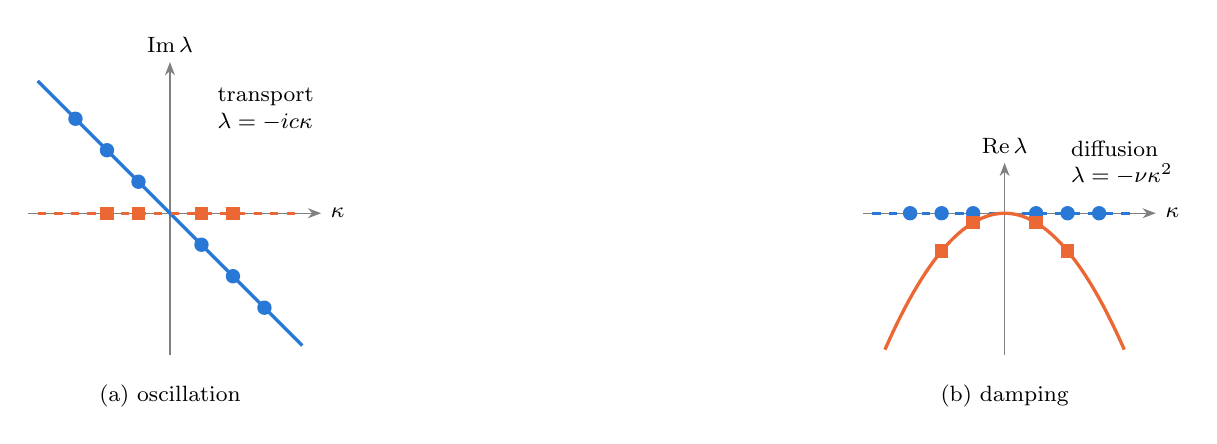
\begin{tikzpicture}[x=0.40cm,y=0.40cm,>=Stealth,font=\footnotesize]
  % (a) oscillation slice
  \begin{scope}
    \draw[->,gray] (-4.5,0)--(4.8,0) node[right,black]{$\kappa$};
    \draw[->,gray] (0,-4.5)--(0,4.8) node[above,black]{$\operatorname{Im}\lambda$};
    \draw[very thick,color={rgb,255:red,42;green,120;blue,214}] (-4.2,4.2)--(4.2,-4.2);
    \draw[very thick,color={rgb,255:red,235;green,104;blue,52},dashed] (-4.2,0)--(4.2,0);
    \foreach \k in {-3,-2,-1,1,2,3} \fill[color={rgb,255:red,42;green,120;blue,214}] (\k,-\k) circle (2.6pt);
    \foreach \k in {-2,-1,1,2} \fill[color={rgb,255:red,235;green,104;blue,52}] (\k,0) +(-2.4pt,-2.4pt) rectangle +(2.4pt,2.4pt);
    \node[anchor=west,align=left] at (1.2,3.3) {transport\\$\lambda=-ic\kappa$};
    \node at (0,-5.8) {(a) oscillation};
  \end{scope}
  % (b) damping slice
  \begin{scope}[xshift=10.6cm]
    \draw[->,gray] (-4.5,0)--(4.8,0) node[right,black]{$\kappa$};
    \draw[->,gray] (0,-4.5)--(0,1.6) node[above,black]{$\operatorname{Re}\lambda$};
    \draw[very thick,color={rgb,255:red,42;green,120;blue,214},dashed] (-4.2,0)--(4.2,0);
    \draw[very thick,color={rgb,255:red,235;green,104;blue,52},domain=-3.8:3.8,samples=60] plot (\x,{-0.3*\x*\x});
    \foreach \k in {-3,-2,-1,1,2,3} \fill[color={rgb,255:red,42;green,120;blue,214}] (\k,0) circle (2.6pt);
    \foreach \k in {-2,-1,1,2} \fill[color={rgb,255:red,235;green,104;blue,52}] (\k,{-0.3*\k*\k}) +(-2.4pt,-2.4pt) rectangle +(2.4pt,2.4pt);
    \node[anchor=west,align=left] at (1.8,1.6) {diffusion\\$\lambda=-\nu\kappa^2$};
    \node at (0,-5.8) {(b) damping};
  \end{scope}
\end{tikzpicture}
\caption{The idea of the paper on the equation $(\partial_t+c\,\partial_x)(\partial_t-\nu\,\partial_x^2)u=0$. Every Fourier mode
$e^{\lambda t+i\kappa x}$ of a solution lies on the zero set of one factor of the symbol $(\tau+c\xi)(\tau-\nu\xi^2)$: circles
on the line of the transport factor, squares on the parabola of the diffusion factor (schematic). Identifying the equation means finding these two groups.}\label{fig:branches}
\end{figure}


\paragraph{How to read the status labels} Each statement carries one of: \proved{} (complete proof, independently reviewed), \modulo{X} (complete except for a cited published theorem~X whose source was checked), \condl{} (depends on an unverified lemma),
\openq{}, or \falsest{} (a counterexample exists). The reviewers were independent AI agents, not human referees; fifteen core algebraic theorems were additionally machine-checked in Lean~4 (branch directory \texttt{proofs/lean}). Grey tags such as \led{C3-T1}
refer to entries of the claim ledger kept with the proofs.

\paragraph{Results at a glance} \Cref{tab:results} lists the main statements; \cref{fig:dependency} shows how they depend on each other. Section~\ref{sec:theory} builds the algebra, \cref{sec:groups} proves the grouping principle and its stability,
\cref{sec:inside} treats the interaction term, \cref{sec:identify} asks when a solution determines its equation, \cref{sec:nonlin} moves to nonlinear equations, and \cref{sec:limits} collects the limits. Proofs are in \cref{app:proofs}; \cref{app:primer} is a primer.

\begin{table}[tbp]
\centering\small
\caption{Main results in the order in which they are proved. ``Proved'' means a complete proof that survived an independent review.}\label{tab:results}
\begin{tabular}{@{}p{2.6cm}p{7.4cm}p{2.6cm}@{}}
\toprule
Topic & Result & Status\\\midrule
Identification & $\Ann(u)=(P)\iff(P/P_i)(\partial)u\notin\EP$ for every irreducible $P_i\mid P$ (\cref{thm:ident}) & \proved\\
Data limits & no finite certificate; black box impossible; decidable with a bound or a holonomic model (\cref{prop:certify}) & \proved\\
Decomposition & $\ker P=\sum_j\ker Q_j$ on simply connected $\Omega$, overlap of dimension $\delta(P)$ (\cref{thm:factor}) & \proved\\
Terms vs.\ factors & a split per additive term is false in general (\cref{prop:terms}) & \proved\\
Stability & the split is stable iff $\gN>0$; for two factors, positive Friedrichs angle (\cref{thm:hm}) & \proved\\
Interaction term & $\Eint=\prod(\Id+\Delta_n)-\Id-\sum\Delta_n$; $O(N)$ value, $\Theta(2^N)$ table (\cref{thm:eint}) & \proved\\
Instability & $u_0\mapsto\Eint$ is not continuous in $H^m$ (\cref{prop:discont}) & \proved\\
Nonlinear & Burgers: closed form before the shock, sharp behaviour across it (\cref{sec:nonlin}) & \proved / \modulo{Kru\v zkov}\\
\bottomrule
\end{tabular}
\end{table}

% Figure (Paper B): how the analytical results depend on each other and where the algorithm uses them.
\begin{figure}[tbp]
\centering
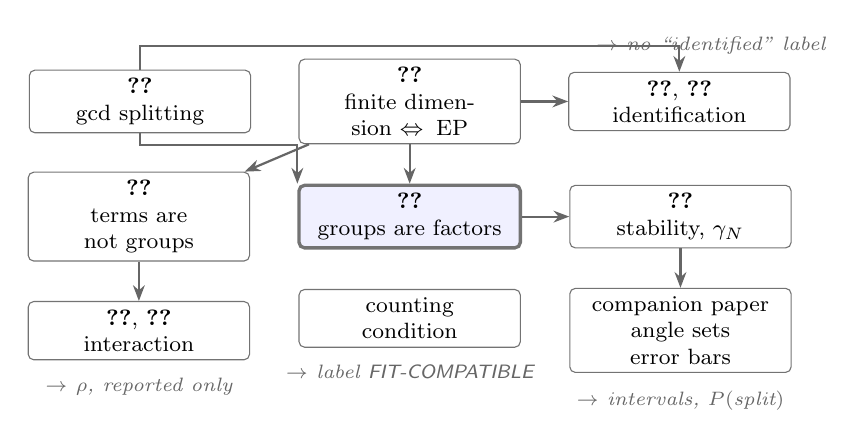
\begin{tikzpicture}[
  node distance=5mm and 6mm,
  res/.style={draw=black!55, rounded corners=2pt, align=center, font=\footnotesize, inner sep=3pt, text width=26mm},
  key/.style={res, fill=blue!6, very thick},
  use/.style={font=\scriptsize\itshape, text=black!60, align=left},
  arr/.style={-{Stealth[length=2mm]}, black!60, thick}]
\node[res] (gcd) {\cref{lem:gcd}\\gcd splitting};
\node[res, right=of gcd] (ep) {\cref{lem:ep}\\finite dimension $\Leftrightarrow\EP$};
\node[res, right=of ep] (ident) {\cref{thm:ident}, \cref{prop:unique}\\identification};
\node[key, below=of ep] (factor) {\cref{thm:factor}\\groups are factors};
\node[res, left=of factor] (terms) {\cref{prop:terms}\\terms are not groups};
\node[res, right=of factor] (hm) {\cref{thm:hm}\\stability, $\gN$};
\node[res, below=of terms] (eint) {\cref{thm:eint}, \cref{prop:discont}\\interaction};
\node[res, below=of hm] (bayes) {companion paper\\angle sets error bars};
\node[res, below=of factor] (count) {counting\\condition};
\draw[arr] (ep)--(ident); \draw[arr] (gcd.north) -- ++(0,3mm) -| (ident.north);
\draw[arr] (gcd.south) -- ++(0,-1.5mm) -| (factor.north west);
\draw[arr] (ep)--(factor); \draw[arr] (ep)--(terms); \draw[arr] (factor)--(hm); \draw[arr] (terms)--(eint); \draw[arr] (hm)--(bayes);
\node[use, below=1mm of eint] {$\to$ $\rho$, reported only};
\node[use, below=1mm of count] {$\to$ label \FC};
\node[use, below=1mm of bayes] {$\to$ intervals, $P(\text{split})$};
\node[use, above=1mm of ident, xshift=4mm] {$\to$ no ``identified'' label};
\end{tikzpicture}
\caption{How the results of \cref{sec:theory} depend on each other (arrows) and where the algorithm uses them
(italic). The shaded result is the grouping principle; everything else either prepares it or measures how well it
can be carried out on finite data.}\label{fig:dependency}
\end{figure}


\section{Derivatives become polynomials}\label{sec:theory}
\inbrief{Before asking what a solution knows, we turn operators into polynomials and solutions into objects that carry an ideal of equations; the one-variable case shows every idea in miniature.}
% Shared module: symbols, the operator ring, annihilators, the intrinsic operator.
\subsection{Derivatives become polynomials}\label{sec:ring}
Throughout, $\Omega\subset\R^2$ is a domain in the variables $(t,x)$ and every operator has constant
coefficients,
\[
  P(\partial_t,\partial_x)=\sum_{j,k}c_{jk}\,\partial_t^{\,j}\partial_x^{\,k},\qquad c_{jk}\in\C .
\]
The exponentials $\psi_{\tau,\xi}(t,x)=e^{\tau t+\xi x}$, $(\tau,\xi)\in\C^2$, are common eigenfunctions of
all such operators: $\partial_t \psi_{\tau,\xi}=\tau \psi_{\tau,\xi}$, $\partial_x \psi_{\tau,\xi}=\xi \psi_{\tau,\xi}$ and
therefore
\begin{equation}\label{eq:symbol-action}
  P(\partial)\,\psi_{\tau,\xi}=P(\tau,\xi)\,\psi_{\tau,\xi}.
\end{equation}
Differentiation is thus replaced by multiplication, and operators are replaced by polynomials.

\begin{definition}[Operator ring, symbol, characteristic variety]\label{def:ring}
The constant-coefficient operators form the commutative ring
$\ring=\C[\partial_t,\partial_x]\cong\C[\tau,\xi]$. The polynomial $P(\tau,\xi)$ is the \emph{symbol} of
$P(\partial)$, and its zero set $\Var(P)=\{(\tau,\xi)\in\C^2:P(\tau,\xi)=0\}$ is the
\emph{characteristic variety}.
\end{definition}

By \eqref{eq:symbol-action}, $\psi_{\tau,\xi}$ solves $P(\partial)u=0$ exactly when $(\tau,\xi)\in\Var(P)$.
A Fourier mode in space is the case $\xi=i\kappa$ with wavenumber $\kappa\in\R$; then
$P(\tau,i\kappa)=0$ is the \emph{dispersion relation}, and the roots $\tau=\lambda(\kappa)$ are the
temporal rates of the mode $e^{\lambda(\kappa)t+i\kappa x}$.

\paragraph{Convention}
We keep the algebraic variable $\xi$ in statements about the ring and write $\xi=i\kappa$ only when we
evaluate on Fourier modes. With this convention a symbol has real coefficients exactly when the
equation is real, and no factor $i$ ever appears inside $\ring$.

\begin{example}[Transport plus diffusion: the running example]\label{ex:tpd}
The operator $P=(\partial_t+c\,\partial_x)(\partial_t-\nu\,\partial_x^2)$, with speed $c>0$ and diffusivity
$\nu>0$, has symbol
\[
  P(\tau,\xi)=Q_1Q_2,\qquad Q_1=\tau+c\,\xi,\qquad Q_2=\tau-\nu\,\xi^2 .
\]
On Fourier modes the two factors give two dispersion branches, $\lambda_1(\kappa)=-ic\kappa$ (a
wave that travels without decay) and $\lambda_2(\kappa)=-\nu\kappa^2$ (a standing mode that decays).
A solution is any superposition of modes on the two branches. The equation is one object; its
\emph{two factors} are two groups of modes. Recovering those groups from data is the subject of this
paper. We use $c=1$, $\nu=0.3$ in all numerical illustrations.
\end{example}

\subsection{What a solution knows: the annihilator}\label{sec:ann}
A single function satisfies many equations: $e^{x}$ is annihilated by $\partial_x-1$, by
$\partial_x^2-1$ and by every multiple of $\partial_x-1$.

\begin{definition}[Annihilator]\label{def:ann}
For a distribution $u$ on $\Omega$, $\Ann(u)=\{Q\in\ring:\ Q(\partial)u=0\}$.
\end{definition}

$\Ann(u)$ is an ideal: it is closed under sums and under multiplication by any operator, because
$(SQ)(\partial)u=S(\partial)\big(Q(\partial)u\big)=0$. It collects every constant-coefficient equation
that $u$ satisfies. We use three classical facts about $\C[\tau,\xi]$~\cite{CLO15}:
unique factorization into irreducible polynomials; B\'ezout's theorem (two polynomials without a
common factor have finitely many common zeros); and Hilbert's Nullstellensatz (if $q$ vanishes on
the zero set $\Var(I)$ of an ideal $I$, then $q^k\in I$ for some $k$). All three require the complex
field, which is why symbols are always considered over $\C$.

\begin{lemma}[Splitting off the greatest common divisor]\label{lem:gcd}
Every nonzero ideal $I\subset\ring$ factors as $I=g\cdot J$, where $g=\gcdop(I)$ and $J$ is an ideal
with finite zero set $\Var(J)$.
\end{lemma}

The proof (\cref{app:proofs}) is elementary: divide by $g$, then use B\'ezout on two elements of $J$
without a common factor. Applied to $I=\Ann(u)$ the lemma gives the decomposition
\begin{equation}\label{eq:GJ}
  \Ann(u)=\Gu\,\Ju,\qquad \Gu=\gcdop\Ann(u),\qquad \sigp(u)=\Var(\Ju)\ \text{finite}.
\end{equation}
The polynomial $\Gu$ is the part of the equation that $u$ fills out along whole curves of $\C^2$;
the finite set $\sigp(u)$, the \emph{point spectrum} of $u$, lists the isolated exponentials that $u$
happens to contain. We call $\Gu$ the \emph{intrinsic operator} of $u$: it depends on $u$ alone,
whereas an annihilator $P$ supplied from outside may contain spurious factors.

\paragraph{Reading the two pieces}
The two objects in~\eqref{eq:GJ} answer different questions. The polynomial $\Gu$ is a differential
equation: its zero set $\Var(\Gu)$ is a union of curves in $\C^2$, and each curve is a continuous family of
exponential modes $e^{\tau t+\xi x}$, all solving $\Gu(\partial)v=0$. The point spectrum $\sigp(u)$ is a list: the
finitely many individual exponential modes that are present in this particular function $u$ and are not
accounted for by $\Gu$. In short, $\Gu$ identifies an equation that describes a whole family of modes;
$\sigp(u)$ identifies the isolated modes that $u$ happens to contain. \Cref{ex:extremes} shows the two
extreme cases.

\begin{example}[Two extremes]\label{ex:extremes}
For $u=e^{x}$, $\Ann(u)=(\tau,\ \xi-1)$ is the ideal of the single point $(0,1)$; hence $\Gu=1$ and
$\sigp(u)=\{(0,1)\}$: the function knows one exponential and no equation. For $u=f(x-ct)$ with a
profile $f$ that is not a finite sum of exponentials times polynomials,
$\Ann(u)=(\tau+c\xi)$; hence $\Gu=\tau+c\xi$ and $\sigp(u)=\emptyset$: the function knows its
equation completely (\cref{thm:ident}).
\end{example}

% Shared module: exponential-polynomials.
\subsection{Exponential-polynomials: the solutions that remember too little}\label{sec:ep}
\begin{definition}[Exponential-polynomials]\label{def:ep}
$\EP$ is the set of finite sums $\sum_{j}p_j(t,x)\,e^{\tau_jt+\xi_jx}$ with polynomials $p_j$ and
exponents $(\tau_j,\xi_j)\in\C^2$. $\EP(\Omega)$ denotes their restrictions to $\Omega$.
\end{definition}

For a function $w$ let $\ring w=\spn\{\partial_t^{\,j}\partial_x^{\,k}w:\ j,k\ge0\}$ be the space of all its
derivatives. The map $Q\mapsto Q(\partial)w$ is onto $\ring w$ with kernel $\Ann(w)$, so
$\ring w\cong\ring/\Ann(w)$ as vector spaces.

\begin{lemma}[Finite-dimension criterion]\label{lem:ep}
Let $\Omega$ be connected. Then $w\in\EP(\Omega)$ if and only if $\dim_\C\ring w<\infty$. In that case
$\Var(\Ann w)$ is the finite set of exponents $\{(\tau_j,\xi_j)\}$ that occur in $w$.
\end{lemma}

\begin{proof}[Proof idea]
We show that $w$ is an exponential-polynomial if and only if its derivatives span a finite-dimensional
space. ($\Rightarrow$) For one term $w=p(t,x)\,e^{at+bx}$,
\[
  \partial_tw=(p_t+a\,p)\,e^{at+bx},\qquad \partial_xw=(p_x+b\,p)\,e^{at+bx}.
\]
Differentiation never raises the degree of $p$, so every derivative of $w$ lies in the finite-dimensional space
of polynomials of degree at most $\deg p$ times $e^{at+bx}$; a finite sum of such terms stays in a finite sum of
such spaces. ($\Leftarrow$) If $\ring w$ is finite-dimensional, $\partial_t$ and $\partial_x$ map it to itself and act
on it as two commuting matrices $A$ and $B$. Their minimal polynomials $m_A$ and $m_B$ give two
constant-coefficient differential equations,
\[
  m_A(\partial_t)\,w=0,\qquad m_B(\partial_x)\,w=0,
\]
one in each variable. On every rectangle inside $\Omega$ their common solutions are exponential-polynomials, and
connectedness extends this representation to all of $\Omega$. The joint eigenvalues $(a,b)$ of $A$ and $B$ are
the exponents that occur in $w$. Details are in \cref{app:proofs}.
\end{proof}

\inbrief{Deciding whether $w\in\EP$ is a finite-dimensional linear-algebra question: compute the rank
of the derivatives of $w$. The joint eigenvalues of the two matrices are the exponents, that is, the
points of $\C^2$ at which $w$ lives. This is the computational core of everything that follows: the
matrix pencil of the companion algorithm paper is exactly this eigenvalue computation, done for $\partial_t$
one wavenumber at a time.}

\begin{example}[Rich and poor solutions of the heat equation]\label{ex:heat-rich-poor}
A single heat mode $e^{-\nu\kappa^2t+i\kappa x}$ and any finite sum of such modes belong to $\EP$.
The heat kernel $t^{-1/2}e^{-x^2/(4\nu t)}$ does not: its $x$-derivatives are polynomials of
increasing degree times the same Gaussian, so they span an infinite-dimensional space.
\end{example}

\sectionbrief
{one variable $x$, an ODE $p(D)u=0$ with constant coefficients, $D=d/dx$, $p$ known.}
{in one variable every object of the later sections (minimal annihilator, spectral projectors, companion matrix) appears with explicit formulas and no geometry of curves.}
{prototype for Section~\ref{sec:ident} (identification) and Section~\ref{sec:groups} (the Lagrange projectors reappear as Eq.~\eqref{xeq:lagrange}).}
This section introduces, in the simplest setting, objects that reappear in Sections~\ref{sec:ident} and~\ref{sec:groups}: the minimal annihilator, the companion matrix and the spectral projectors.

\begin{notebox}{Setting and symbols}
\begin{itemize}[nosep]
\item We consider an ODE $p(D)u=0$ in one variable $x$, with $D=d/dx$ (in this section only; elsewhere $D$ is a diffusion constant).
\item The polynomial $p(\lambda)=\prod_j(\lambda-\lambda_j)^{m_j}$ has distinct roots $\lambda_j\in\C$ with multiplicities $m_j\ge1$, so that $m=\deg p=\sum_jm_j$ is the \emph{order} of the equation (not to be confused with the Sobolev index $m$ of Section~\ref{sec:groups}).
\item The set of solutions is the \emph{kernel} $\ker p(D)$, and
\[
\ker p(D)=\Big\{\sum_jq_j(x)e^{\lambda_jx}:\ \deg q_j<m_j\Big\},
\]
where each $q_j$ is a polynomial of degree $<m_j$.
\end{itemize}
\end{notebox}

\begin{aside}{Why this form}
For one root, $(D-\lambda)\big(q\,e^{\lambda x}\big)=q'e^{\lambda x}$: applying $D-\lambda$ lowers the degree of $q$ by one. Hence $(D-\lambda_j)^{m_j}$ kills $q\,e^{\lambda_jx}$ exactly when $q^{(m_j)}=0$, i.e.\ $\deg q<m_j$.

Each root therefore contributes the $m_j$ functions $x^ke^{\lambda_jx}$ ($0\le k<m_j$): these are the natural basis functions of the equation, finitely many, and together they form a basis of $\ker p(D)$, a space of dimension $m$.
\end{aside}

\begin{aside}{Example}
$p(\lambda)=(\lambda-1)^2(\lambda+2)^3$ has $\lambda_1=1$, $m_1=2$, $\lambda_2=-2$, $m_2=3$, order $m=5$. A basis of the solutions is
\[
e^{x},\quad xe^{x},\quad e^{-2x},\quad xe^{-2x},\quad x^2e^{-2x},
\]
so every solution is
\[
c_1e^{x}+c_2xe^{x}+c_3e^{-2x}+c_4xe^{-2x}+c_5x^2e^{-2x}.
\]
\end{aside}

\subsection{Identification by the Wronskian}
\begin{proposition}[{(ODE identification)}]
Let $u\in\ker p(D)$. The minimal annihilator of $u$ has degree equal to the number of independent basis functions actually present in $u$; it equals $p$ if and only if $u,u',\dots,u^{(m-1)}$ are linearly independent (nonvanishing Wronskian), i.e.\ iff every root of $p$ appears in $u$ with its full multiplicity.
\end{proposition}
\emph{Reason.} $\dimc\spn\{u,u',u'',\dots\}$ is the degree of the minimal annihilator (Lemma~\ref{lem:ep} in one variable); a missing root lowers it.

\subsection{The companion matrix and spectral form}
Write $p(\lambda)=\lambda^m+a_{m-1}\lambda^{m-1}+\dots+a_0$ (monic) and put $X=(u,u',\dots,u^{(m-1)})^{\top}$. Then $X'=CX$ with
\[
C=\begin{pmatrix}0&1&&\\&0&\ddots&\\&&\ddots&1\\-a_0&-a_1&\cdots&-a_{m-1}\end{pmatrix},\qquad
X(x)=e^{xC}X(0).
\]
The eigenvalues of $C$ are the roots of $p$. For distinct roots the matrix exponential has the spectral form
\begin{equation}\label{eq:spectral}
\begin{aligned}
e^{xC}&=\sum_{j=1}^me^{\lambda_jx}\,\Pi_j,\\
\Pi_j&=\prod_{k\ne j}\frac{C-\lambda_k\Id}{\lambda_j-\lambda_k},
\end{aligned}
\end{equation}
where the $\Pi_j$ are the Lagrange projectors onto the eigenspaces. The last row of $C$ carries the whole equation; $C$ is a \emph{matrix over the base field} for an ODE, but, as soon as the coefficients depend on $x$, or there is a second variable, its last row has entries that are operators and the object becomes a matrix over a noncommutative or polynomial ring. The invariant statement is that the whole equation corresponds to the cyclic module $\ring/\Ann(u)$ (Section~\ref{sec:theory}); the companion matrix is a way to compute with it relative to one chosen direction.

\begin{proposition}[{(Projectors of the companion matrix) \led{II-T2} \proved[]}]
The projectors $\Pi_j$ are explicit rational functions of the coefficients, with poles exactly where roots collide; they are polynomial in the coefficients if and only if the corresponding varieties are disjoint. They are \emph{not} orthogonal in general: the companion matrix is not normal for $m=2$ \falsest{} (the contrary was an early conjecture).
\end{proposition}
Hence Hilbert-space orthogonality arguments need an inner product adapted to the problem, not the standard one on the coefficient vector.

\subsection{Tensor construction versus module construction}
One may encode a PDE in a higher-order tensor of derivatives, $J=\partial_{x_{i_1}}\otimes\cdots\otimes\partial_{x_{i_n}}$, or by the companion form. The comparison, \led{Gate 3}: the \emph{principal symbol tensor} $\sigma_m(P)\in\mathrm{Sym}^m(\C^2)$ only sees the highest-order part of $P$ (for the heat operator it sees $\xi^2$ alone), so it is an invariant ``at infinity''; the \emph{cyclic module} $\ring/\Ann(u)$ is the complete invariant. All subsequent results use the module.

\begin{keypoint}
This section shows how an ODE's polynomial encodes its solution space. Its roots determine the exponential rates, their multiplicities determine the polynomial prefactors, the companion matrix represents differentiation, and spectral projectors isolate the different modes. The later sections generalize these ideas to multiple commuting derivatives, where the same structure survives but requires more algebraic machinery: the minimal annihilator becomes the ideal $\Ann(u)$ (Section~\ref{sec:ident}) and the Lagrange projectors reappear as Eq.~\eqref{xeq:lagrange} (Section~\ref{sec:groups}).
\end{keypoint}

%======================================================================


\section{Groups are factors, not terms}\label{sec:groups}
\inbrief{The factor decomposition, its stability measured by an angle, and the regularity of the components.}
% Shared module: the grouping theorem (factor decomposition), projectors, why terms fail, holes.
\subsection{Groups are factors, not terms}\label{sec:factor}
Suppose the operator is known and factored as
\begin{equation}\label{eq:factored}
  P=P_1^{e_1}\cdots P_N^{e_N},\qquad Q_j=P_j^{e_j}\ \text{pairwise coprime}.
\end{equation}
Two ways of splitting a solution suggest themselves: one piece per \emph{factor} $Q_j$, or one piece
per additive \emph{term} of the operator (for $u_t=\nu u_{xx}-cu_x$, one piece for diffusion and one
for transport). Only the first works.

\begin{theorem}[Factor decomposition]\label{thm:factor}
Let $\Omega\subset\R^2$ be bounded, connected and simply connected, and let $P$ be as in
\eqref{eq:factored}. Every $u\in\ker P(\partial)$ (in $\mathcal D'(\Omega)$ or $C^\infty(\Omega)$) can be
written
\begin{equation}\label{eq:decomp}
  u=\sum_{j=1}^N u_j,\qquad Q_j(\partial)\,u_j=0 .
\end{equation}
The tuples $(u_1,\dots,u_N)$ that sum to zero form a space of exponential-polynomials of dimension
exactly
\begin{equation}\label{eq:deltaP}
  \deltaP=\sum_{i<j}\dim_\C\ring/(Q_i,Q_j),
\end{equation}
the number of intersection points of the varieties $\Var(Q_i)$, counted pair by pair and with multiplicity.
\end{theorem}

The number $\dim_\C\ring/(Q_i,Q_j)$ therefore has two readings at once. Geometrically it counts the points where
the curves $\Var(Q_i)$ and $\Var(Q_j)$ meet, with multiplicity. Analytically it is the dimension of the space of
exponential-polynomials that solve both $Q_i$ and $Q_j$, one exponential for each meeting point (times polynomials at a
point of higher multiplicity). For two groups these are exactly the functions that can be moved from one group to the
other without changing $u$: each meeting point of the two curves is one shared mode. For three or more groups $\deltaP$
still gives the dimension of the ambiguity, but the ambiguous tuples need not be sums of modes shared by pairs.

In one variable the statement is B\'ezout's identity: if $aQ_1+bQ_2=1$, then
$u=bQ_2u+aQ_1u$ splits $u$ into a solution of $Q_1$ and a solution of $Q_2$. In two variables
``coprime'' no longer gives $1\in(Q_1,Q_2)$; it only gives finitely many common zeros, and the
finite-dimensional quotient $\ring/(Q_1,Q_2)$ measures exactly how much the two groups overlap. The
proof combines the exact sequence
$0\to\ring/(Q_1Q_2)\to\ring/(Q_1)\oplus\ring/(Q_2)\to\ring/(Q_1,Q_2)\to0$ with the vanishing of the obstruction
$\operatorname{Ext}^1(M,C^\infty(\Omega))$ for the finite-dimensional module $M=\ring/(Q_1,Q_2)$, which reduces to
$H^1_{dR}(\Omega)=0$ (compare the fundamental principle of Ehrenpreis and Palamodov~\cite{Ehr70,Pal70});
see \cref{app:proofs}.

\begin{example}[Running example: two groups with a two-dimensional overlap]\label{ex:tpd-factor}
For $Q_1=\tau+c\xi$ and $Q_2=\tau-\nu\xi^2$ the common zeros are $(0,0)$ and $(c^2/\nu,-c/\nu)$,
both simple, so $\deltaP=2$. The ambiguity is spanned by the constant function and by
$e^{(c^2/\nu)t-(c/\nu)x}$: a constant (or that growing exponential) can be moved from one group to
the other without changing $u$. Among Fourier modes ($\xi=i\kappa$, $\kappa\in\R$) only the
first point is visible: the $\kappa=0$ mode belongs to both groups.
\end{example}

\paragraph{Projectors from the eigenvalues}
When each factor is an evolution factor, $Q_j=\tau-\Lambda_j(\xi)$ with pairwise distinct branches
$\Lambda_j$, a component is an eigenfunction of $\partial_t$: $\partial_tu_j=\Lambda_j(\partial_x)u_j$. Applying
$\prod_{k\ne j}(\partial_t-\Lambda_k(\partial_x))$ to $u=\sum_lu_l$ removes every $u_l$ with $l\ne j$ and multiplies $u_j$ by $\prod_{k\ne j}(\Lambda_j-\Lambda_k)(\partial_x)$.
On a spatial Fourier mode $\kappa$ at which no two branches meet this factor is a nonzero number, hence
\begin{equation}\label{eq:lagrange}
  \hat u_j=\prod_{k\ne j}\frac{\partial_t-\Lambda_k(i\kappa)}{\Lambda_j(i\kappa)-\Lambda_k(i\kappa)}\;\hat u(t,\kappa) .
\end{equation}
This is a multiplier, rational in $\kappa$, with poles exactly where two branches
meet ($\Lambda_j(i\kappa)=\Lambda_k(i\kappa)$), that is, at the visible part of the overlap counted by $\deltaP$.
Formula~\eqref{eq:lagrange} is the Lagrange interpolation formula for the spectral projectors of a
matrix with distinct eigenvalues, applied to $\partial_t$ restricted to one wavenumber: the
\emph{eigenvalues decide the groups}. For the running example,
$\hat u_1(t,\kappa)=\big(\partial_t+\nu\kappa^2\big)\hat u/\big(\nu\kappa^2-ic\kappa\big)$, which is
singular only at $\kappa=0$.

\paragraph{Why additive terms do not form groups}
\begin{proposition}[Terms do not give components]\label{prop:terms}
If $P=\mathcal A_1+\mathcal A_2$ with constant coefficients, then
$\ker P\cap(\ker \mathcal A_1+\ker \mathcal A_2)\subseteq\ker P\cap\ker(\mathcal A_1\mathcal A_2)$, and the right-hand side is
finite-dimensional whenever $\Var(\mathcal A_1)\cap\Var(\mathcal A_2)$ is finite.
\end{proposition}

\begin{proof}
If $u=a+b$ with $\mathcal A_1a=0$ and $\mathcal A_2b=0$, then $\mathcal A_1\mathcal A_2u=\mathcal A_2\mathcal A_1a+\mathcal A_1\mathcal A_2b=0$ because the operators commute.
At a common zero of $P$ and $\mathcal A_1\mathcal A_2$ either $\mathcal A_1=0$, and then $\mathcal A_2=P-\mathcal A_1=0$, or $\mathcal A_2=0$ and then
$\mathcal A_1=0$; so $\Var(P,\mathcal A_1\mathcal A_2)=\Var(\mathcal A_1)\cap\Var(\mathcal A_2)$. When this set is finite, the ideal $(P,\mathcal A_1\mathcal A_2)$
has finite codimension, its common kernel consists of exponential-polynomials with exponents in that
set (\cref{lem:ep}), and it is finite-dimensional.
\end{proof}

For the heat equation, $\mathcal A_1=\partial_t$ and $\mathcal A_2=-\nu\partial_x^2$: every sum $f(x)+a(t)+b(t)x$ of a
solution of $\mathcal A_1$ and one of $\mathcal A_2$ is killed by $\mathcal A_1\mathcal A_2\sim\partial_t\partial_x^2$, while a heat mode
$e^{-\nu\kappa^2t}\cos\kappa x$ is not. A generic heat solution is \emph{not} ``a diffusion part plus a
stationary part''. The leftover of any term-wise split is the interaction term of
\cref{sec:eint}.

\paragraph{Where the decomposition fails}
The hypotheses of \cref{thm:factor} are not technical. On a disconnected domain different pieces
can satisfy different equations. On a domain with a hole the decomposition can fail: the Laplacian
factors as $(\partial_x+i\partial_y)(\partial_x-i\partial_y)$, yet $\log\abs{z}^2$ is harmonic on an annulus
and is not a sum of a holomorphic and an antiholomorphic single-valued function. The obstruction is
the first de Rham cohomology of $\Omega$, which is why the algorithm works on rectangles.

\roleinalg{\Cref{thm:factor} is the grouping principle of the paper. The objects that a learning
algorithm should group are \emph{modes of the same factor}; equivalently, points of the data's
Fourier--Laplace spectrum lying on the same irreducible component of $\Var(P)$. The overlap $\deltaP$
is the irreducible amount of ambiguity, and the algorithm resolves it by a fixed convention
(the companion algorithm paper).}

% Shared module: conditioning of the split, Friedrichs angle, regularity.
\subsection{How well separated are the groups? The Friedrichs angle}\label{sec:cond}
\Cref{thm:factor} is algebraic: it says that the split exists, not that it is stable. Stability is a
geometric property of the component spaces $M_j=\ker_{\Hs}Q_j$, the solutions of each factor in the
Sobolev space $\Hs(\Omega)$. Let
\[
  \sumop:\ \textstyle\bigoplus_{j=1}^N M_j\to\Hs(\Omega),\qquad \sumop(u_1,\dots,u_N)=\sum_ju_j,
\]
be the \emph{sum operator}, with $\norm{(u_1,\dots,u_N)}^2=\sum_j\norm{u_j}_{\Hs}^2$, and define the
\emph{conditioning constant}
\begin{equation}\label{eq:gammaN}
  \gN=\inf_{0\ne v\perp\ker\sumop}\frac{\norm{\sumop v}^2}{\norm{v}^2}
  =\inf\sigma\big(\sumop^*\sumop\big|_{(\ker\sumop)^\perp}\big).
\end{equation}
It is the worst case, over all tuples of pieces, of the size of the sum relative to the size of the
pieces. Tuples in $\ker\sumop$ (the overlap of \cref{thm:factor}) are excluded. By the triangle and Cauchy--Schwarz inequalities,
$\norm{\sum_ju_j}^2\le\big(\sum_j\norm{u_j}\big)^2\le N\sum_j\norm{u_j}^2$, hence
\[
  0\le\gN\le N .
\]
If the spaces are mutually orthogonal, $\norm{\sum_ju_j}^2=\sum_j\norm{u_j}^2$ and $\gN=1$. At the other end, if $M_2$
approaches $M_1$ one can take $u_2\approx-u_1$: the pieces stay of unit size while their sum becomes arbitrarily
small, so $\gN\to0$. A small $\gN$ is the signature of groups that can almost cancel each other.

For two groups, $\gamma_2=1-\cF$, where the \emph{Friedrichs cosine}
\[
  \cF=\sup\big\{\abs{\ip ab}:\ a\in M_1\ominus(M_1\cap M_2),\ b\in M_2\ominus(M_1\cap M_2),\
  \norm a=\norm b=1\big\}=\cos\thetaF
\]
is the cosine of the smallest nonzero angle $\thetaF$ between the two spaces
(\cref{fig:friedrichs})~\cite{Deu01}. In regression terms, $M_1$ and $M_2$ are two blocks of regressors and $\cF$ is the
largest correlation between a combination of the first block and one of the second: the closer the blocks are to
collinear, the less the data can attribute to each.

\begin{theorem}[Stability of the split]\label{thm:hm}
Every $u\in\ker_{\Hs}P$ has components $u_j\in\Hs$ if and only if $\sum_jM_j$ is closed and dense in
$\ker_{\Hs}P$. Closedness is equivalent to $\gN>0$, and then
\begin{equation}\label{eq:stability}
  \Big(\sum_j\norm{u_j}_{\Hs}^2\Big)^{1/2}\le\gN^{-1/2}\,\norm{u}_{\Hs}
\end{equation}
for the minimum-norm components. If the component spaces are finite-dimensional, as for the sampled
kernels used by the algorithm, the sum is always closed and density holds whenever the sampled kernel of
$P$ is spanned by those of its factors, so stability reduces to $\gN>0$.
\end{theorem}

Density in $\Hs$ is a genuine condition on infinite-dimensional spaces. On convex domains solutions of
$P(\partial)u=0$ are limits of exponential solutions, uniformly on compact subsets~\cite{Mal56,Hor90},
and every exponential solution lies in $\sum_jM_j$; whether this extends to the $\Hs$ norm up to the boundary
for general $P$ we do not claim.

Two warnings come with the theorem. First, $\gN>0$ can fail on infinite-dimensional component spaces: the pieces of a smooth $u$ may then be
one derivative rougher than $u$ itself. Second, for $N\ge3$ groups the pairwise cosines do not
determine $\gN$: two pairs can be well separated while the three spaces are nearly dependent, so the
full Gram operator of $\sumop$ must be used.

\begin{figure}[tbp]
\centering
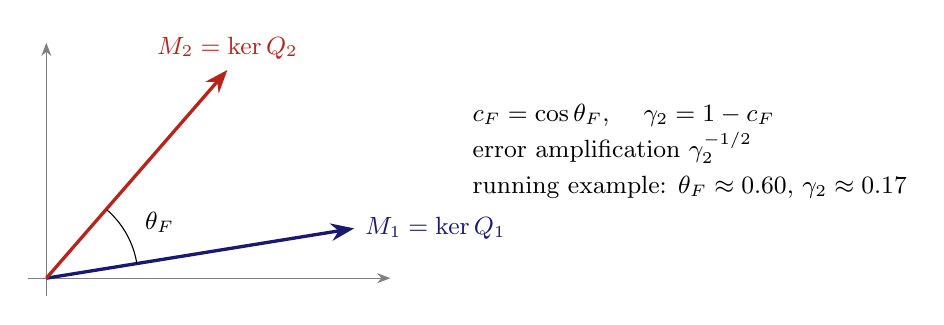
\begin{tikzpicture}[scale=1.15,>=Stealth]
  \draw[->,gray] (-0.2,0)--(3.8,0); \draw[->,gray] (0,-0.2)--(0,2.6);
  \draw[very thick,->,color=MidnightBlue] (0,0)--(3.4,0.55) node[right]{\small $M_1=\ker Q_1$};
  \draw[very thick,->,color=BrickRed] (0,0)--(2.0,2.3) node[above]{\small $M_2=\ker Q_2$};
  \draw (1.0,0.16) arc (9.2:49:1.0); \node at (1.25,0.62) {\small$\thetaF$};
  \node[anchor=west,align=left,font=\small] at (4.6,1.4)
   {$\cF=\cos\thetaF$, \quad $\gamma_2=1-\cF$\\[2pt]
    error amplification $\gamma_2^{-1/2}$\\[2pt]
    running example: $\thetaF\approx0.60$, $\gamma_2\approx0.17$};
\end{tikzpicture}
\caption{The Friedrichs angle $\thetaF$ between the solution spaces of two factors. A small angle
means that large pieces can almost cancel, so recovering the pieces from their sum amplifies errors by
up to $\gamma_2^{-1/2}=(1-\cos\thetaF)^{-1/2}$. The values quoted are those measured on the running
example in the companion algorithm paper.}\label{fig:friedrichs}
\end{figure}

\roleinalg{$\gN$ is computed on the sampled kernel bases and reported with every result.
It enters twice: as the error amplification $\gN^{-1/2}$ of the components, and through the Bayesian
split layer (the companion algorithm paper), whose credible intervals widen and whose split probability
returns to the prior as $\thetaF\to0$. A small angle is therefore never hidden: it shows up as wide
intervals, not as a confident but wrong split.}

\subsection{An explicit projector for evolution factors}
For an evolution operator with $P=\prod_{j=1}^N(\tau-a_j(\xi))$ and distinct $a_j$, a component is an eigenfunction of $\partial_t$: $\partial_tu_j=a_j(\partial_x)u_j$. Applying $\prod_{k\ne j}(\partial_t-a_k(\partial_x))$ to $u=\sum_lu_l$ kills every $u_l$ with $l\ne j$ (it contains the factor $\partial_t-a_l$) and multiplies $u_j$ by $\prod_{k\ne j}(a_j-a_k)(\partial_x)$. Hence
\begin{equation}\label{xeq:lagrange}
u_j=\prod_{k\ne j}\frac{\partial_t-a_k(\partial_x)}{a_j(\partial_x)-a_k(\partial_x)}\;u ,
\end{equation}
the Lagrange formula of Eq.~\eqref{eq:spectral} with $C$ replaced by $\partial_t$. The result is a Fourier multiplier in $x$ that is rational in $\xi$, with poles where $a_j(\xi)=a_k(\xi)$; this matches the characterization ``projectors rational in $\xi$ iff the factors are coprime'' \led{II-T2/T3}.

\subsection{Where decomposition fails}
\begin{proposition}[{(Holes) \led{C12-P10} \proved[]}]
On a domain with a hole, the decomposition fails for some $P$.
\end{proposition}
Figure~\ref{fig:hole} shows the standard obstruction. In the theorem the hypothesis ``simply connected'' means $H^1_{dR}(\Omega)=0$, exactly what removes this obstruction; a cohomological criterion for non-simply connected $\Omega$ is also available \led{OP-FUN, C12-Q6}.
\begin{figure}[!htb]
\centering
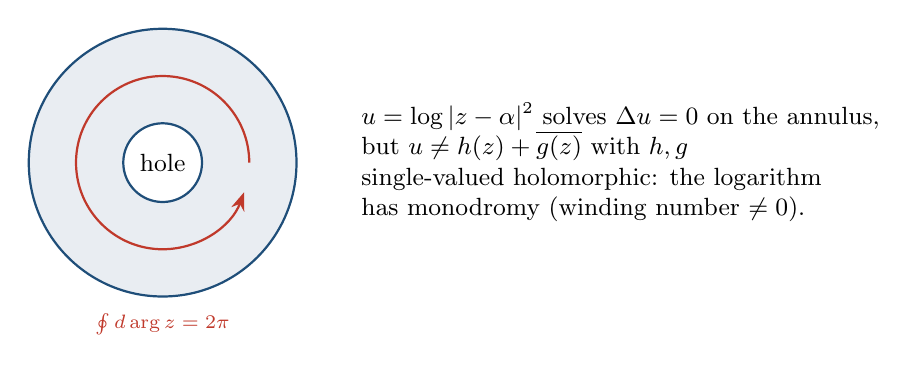
\begin{tikzpicture}
\fill[cA!10] (0,0) circle (1.7); \fill[white] (0,0) circle (0.5);
\draw[cA,thick] (0,0) circle (1.7); \draw[cA,thick] (0,0) circle (0.5);
\node at (0,0) {\small hole};
\draw[cB,thick,-{Stealth}] (1.1,0) arc (0:340:1.1);
\node[cB,font=\scriptsize] at (0,-2.05) {$\oint d\arg z=2\pi$};
\node[align=left,font=\small,anchor=west] at (2.4,0) {$u=\log|z-\alpha|^2$ solves $\Delta u=0$ on the annulus,\\ but $u\neq h(z)+\overline{g(z)}$ with $h,g$\\ single-valued holomorphic: the logarithm\\ has monodromy (winding number $\neq0$).};
\end{tikzpicture}
\caption{The Laplacian $\partial_x^2+\partial_y^2=(\partial_x+i\partial_y)(\partial_x-i\partial_y)$ factors, but the factor decomposition fails on a punctured disc: the obstruction is topological ($H^1_{dR}\neq0$).}\label{fig:hole}
\end{figure}

\subsection{Regularity: when are the components in $H^m$?}
The decomposition is an algebraic statement; analysis enters when we want components in a Sobolev space. For two components the governing condition is geometric: the two component spaces $M_1$ and $M_2$ must be separated by a positive angle (Figure~\ref{xfig:friedrichs}); the next theorem makes this precise for any number of components. Two difficulties appear along the way; they are collected in the box after the theorem.
\begin{proposition}[{(Loss of a derivative) \led{C12-C1} \falsest}]\label{prop:loss}
``If $u\in H^m(\Omega)$ then all $u_j\in H^m$'' is false: one derivative can be lost. In other words, the pieces of a smooth function may be rougher than the function itself.
\end{proposition}
\begin{theorem}[{(Regularity criterion) \led{C12-T3, C12-P7} \proved[]}]\label{xthm:hm}
All components lie in $H^m$ for every $u\in\ker_{H^m}P$ iff the sum $\sum_j\ker_{H^m}Q_j$ is \emph{closed} and \emph{dense} in $\ker_{H^m}P$. Closedness is equivalent to $\gamma_N>0$, where
\[
\begin{aligned}
\gamma_N&=\inf\sigma\big(S^*S\big|_{(\ker S)^\perp}\big),\\
S&:\bigoplus_{j=1}^N\ker Q_j\to H^m,\qquad S(u_1,\dots,u_N)=\sum_{j=1}^Nu_j .
\end{aligned}
\]
For $N=2$ this is the condition $c_F<1$ on the Friedrichs cosine. Density holds on every bounded convex $\Omega$, for every $P$ and $m$ \led{OPF5B-T1} \modulo{H\"ormander~\cite{ho}, Stein}.
\end{theorem}
\begin{notebox}{Reading $\gamma_N$}
\begin{itemize}[nosep]
\item The space $\bigoplus_j\ker Q_j$ consists of the $N$-tuples $v=(u_1,\dots,u_N)$ with norm $\|v\|^2=\sum_j\|u_j\|_{H^m}^2$;
\item $Sv=\sum_ju_j$ is their sum;
\item $S^*$ is the adjoint of $S$;
\item $(\ker S)^\perp$ removes the tuples that sum to zero (the ambiguity of Theorem~\ref{thm:factor});
\item $\inf\sigma$ is the bottom of the spectrum.
\end{itemize}
Since $S^*S$ restricted to $(\ker S)^\perp$ is self-adjoint and nonnegative, the bottom of its spectrum is the minimum of the Rayleigh quotient
\[
\frac{\langle S^*Sv,v\rangle}{\|v\|^2}=\frac{\|Sv\|^2}{\|v\|^2}.
\]
Hence the formula of the theorem is equivalent to the more intuitive
\[
\boxed{\ \gamma_N=\inf_{\substack{v\in(\ker S)^\perp\\ v\ne0}}\frac{\|Sv\|_{H^m}^2}{\|v\|^2}\ }
\]
\end{notebox}

\begin{aside}{In words}
$\gamma_N$ is the worst case, over all tuples of pieces, of the ratio between the size of the sum and the size of the pieces.
\begin{itemize}[nosep]
\item If $\gamma_N>0$ the pieces cannot nearly cancel each other, and
\[
\|v\|\le\gamma_N^{-1/2}\|Sv\|:
\]
the pieces are controlled by the sum, so recovering them from $u$ is stable.
\item If $\gamma_N\to0$ there are large pieces whose sum is tiny, and the recovery is unstable.
\end{itemize}
\textbf{The case $N=2$.} One finds $\gamma_2=1-c_F$, where
\[
c_F=\sup\{|\langle a,b\rangle|:\ a\in M_1\ominus(M_1\cap M_2),\ b\in M_2\ominus(M_1\cap M_2),\ \|a\|=\|b\|=1\}
\]
is the Friedrichs cosine: the part of $v$ lying in $M_1\cap M_2$ contributes the ratio $2$ and does not affect the infimum, and on the rest
\[
\|a+b\|^2\ge(1-c_F)(\|a\|^2+\|b\|^2)
\]
with near-equality attained. Hence $c_F<1\iff\gamma_2>0$, as stated.
\end{aside}
\begin{figure}[!htb]
\centering
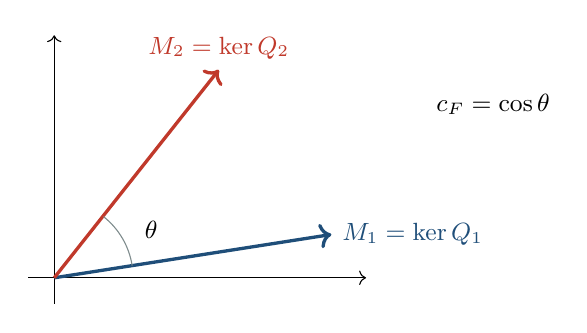
\begin{tikzpicture}[scale=1.1]
\draw[->] (-0.3,0)--(3.6,0); \draw[->] (0,-0.3)--(0,2.8);
\draw[cA,very thick,->] (0,0)--(3.2,0.5) node[right,font=\small]{$M_1=\ker Q_1$};
\draw[cB,very thick,->] (0,0)--(1.9,2.4) node[above,font=\small]{$M_2=\ker Q_2$};
\draw[cG] (0.9,0.14) arc (8.9:51.6:0.9); \node[font=\small] at (1.12,0.55) {$\theta$};
\node[font=\small,anchor=west] at (4.3,2.0) {$c_F=\cos\theta$};



\end{tikzpicture}
\caption{Friedrichs angle $\theta$ between two component spaces $M_1=\ker Q_1$ and $M_2=\ker Q_2$. A larger angle means a better-conditioned recovery of the pieces from their sum.}\label{xfig:friedrichs}
\end{figure}
For $N=2$, Figure~\ref{xfig:friedrichs} reads as follows: $c_F=\cos\theta$; if $\theta>0$ the sum $M_1+M_2$ is closed and the pieces depend continuously on $u$; as $\theta\to0$ the split becomes unstable. For $N\ge3$ the pairwise angles do not suffice; $\gamma_N$, the smallest nonzero eigenvalue of $S^*S$, is the right conditioning number: it is the conditioning of the linear map ``components $\mapsto$ sum'', exactly like the smallest nonzero singular value in a least-squares problem.

\begin{caution}[title=Two problems with regularity]
\textbf{Problem 1: stability \falsest.} Algebraically the split always exists (Theorem~\ref{thm:factor}), but the pieces may be less regular than $u$. When the angle between the component spaces tends to $0$ (that is, $\gamma_N\to0$) the map ``$u\mapsto$ pieces'' becomes unstable, and one derivative can be lost (Proposition~\ref{prop:loss}). For the algorithm: check $\gamma_N>0$ before using the components in $H^m$ (Step~5).\\[3pt]
\textbf{Problem 2: three or more components \openq.} For $N\ge3$ the pairwise cosines $c_F(i,j)$ do not decide whether the sum of kernels is closed: an abstract Hilbert-space counterexample exists \led{S-CHECK-4}, and whether it can occur for differential operators is open \led{C12-Q2}.
\end{caution}

\begin{takeaway}
Algebraically the split always exists (Theorem~\ref{thm:factor}); analytically, the components are well behaved exactly when the component spaces are separated by a positive angle (Theorem~\ref{xthm:hm}). The next section stops asking for a split into factors and asks what survives when one splits by additive terms instead.
\end{takeaway}

%======================================================================


\section{Inside one group: the interaction term}\label{sec:inside}
\inbrief{What remains when a factor is built from several terms: an exact formula, its cost, its instability, and what happens when the terms do not commute.}
% Shared module: interaction term and energy.
\subsection{Inside one group: the interaction term and its energy}\label{sec:eint}
A single factor may have several additive terms: $Q_2=\tau-\nu\xi^2$ has one, but the advection--diffusion
factor $\tau+c\xi-\nu\xi^2$ has two. \Cref{prop:terms} says that such a factor cannot be split further
into one solution per term. We now measure exactly what is left over.

Consider an evolution $u_t=\mathcal Au$ with $\mathcal A=\mathcal A_1+\dots+\mathcal A_K$ (the terms), the flow $\flow(t)=e^{t\mathcal A}$ and the
flows of the single terms $\flow_n(t)=e^{t\mathcal A_n}$. If term $n$ acted alone it would change the datum by
$\Delta_nu_0=(\flow_n(t)-\Id)u_0$. The \emph{interaction term} is the part of the evolution that is not
the sum of these single-term changes,
\begin{equation}\label{eq:eint-def}
  \Eint(t)=u(t)-u_0-\sum_{n=1}^K\big(\flow_n(t)u_0-u_0\big).
\end{equation}

\begin{theorem}[Interaction term]\label{thm:eint}
If the terms commute (in particular, for constant coefficients),
\[
  \Eint(t)=\Big[\prod_{n=1}^K(\Id+\Delta_n)-\Id-\sum_{n=1}^K\Delta_n\Big]u_0
  =\sum_{\mathcal E\subseteq\{1,\dots,K\},\ \abs{\mathcal E}\ge2}\Big(\prod_{n\in\mathcal E}\Delta_n\Big)u_0 .
\]
For two terms $\Eint=\Delta_1\Delta_2u_0$. On Fourier modes, with symbols $\hat{\mathcal A}_n(\kappa)$ of the terms,
\begin{equation}\label{eq:eint-fourier}
  \widehat{\Eint}(t,\kappa)=\Big[\prod_ne^{t\hat{\mathcal A}_n(\kappa)}-1-\sum_n\big(e^{t\hat{\mathcal A}_n(\kappa)}-1\big)\Big]\hat u_0(\kappa).
\end{equation}
\end{theorem}

\begin{proof}
Commuting terms give $\flow=\prod_n\flow_n=\prod_n(\Id+\Delta_n)$. Expanding the product over subsets
$\mathcal E\subseteq\{1,\dots,K\}$ and removing the subsets with zero or one element gives the formula; on
Fourier modes every operator is multiplication by a number.
\end{proof}

Formula~\eqref{eq:eint-fourier} costs $O(K)$ operations per wavenumber, although writing out all
cross terms would need $2^K-K-1$ of them. For advection--diffusion,
$\abs{\widehat{\Eint}}/\abs{\hat u_0}=\abs{(e^{-ic\kappa t}-1)(e^{-\nu\kappa^2t}-1)}\le2$: the interaction
is of the same size as the solution, so it is not a small correction that a regularizer could remove.

\begin{proposition}[No stable removal]\label{prop:discont}\label{thm:noreg}\label{thm:nocont}
Let $Q=\tau+c\xi-\nu\xi^2$ (advection--diffusion, terms $-c\partial_x$ and $\nu\partial_x^2$) on a bounded
rectangle $\Omega=(0,T)\times(a,b)$. For every $s\ge0$,
\[
  \sup\Big\{\norm{\Eint}_{L^2(\Omega)}/\norm{u}_{\Hs(\Omega)}:\ u\in\EP,\ Q(\partial)u=0,\ u\ne0\Big\}=\infty,
\]
so $u\mapsto\Eint$ has no continuous extension to $\ker_{\Hs}Q$. Moreover, a solution of $Q(\partial)u=0$ is a
sum $v+w$ of solutions of the single-term evolutions $(\partial_t+c\partial_x)v=0$ and $(\partial_t-\nu\partial_x^2)w=0$ only
if it lies in a finite-dimensional space of exponential-polynomials.
\end{proposition}

The test solutions are $e^{\lambda_\zeta t+\zeta x}$ with real $\zeta>c/\nu$ and $\lambda_\zeta=\nu\zeta^2-c\zeta$, legitimate
data on a bounded interval: diffusion alone amplifies them by $e^{\nu\zeta^2t}$, the solution grows only like
$e^{\lambda_\zeta t}$, and the interaction must cancel a difference that grows faster than any power of $\zeta$
(\cref{app:proofs}). On a periodic domain with bounded wavenumbers the Fourier multiplier above is bounded by
$2$; the instability comes from the non-periodic window, which is the situation of real data. The second
statement means that a model which writes the data as a sum of single-term pieces, with any penalty on the
pieces, leaves a remainder on generic data, and that remainder is the interaction.

\paragraph{Energy}
We measure the size of a group and of the interaction by $L^2$ energies on the observation window.
The \emph{energy share} of group $j$ and the \emph{interaction ratio} are
\begin{equation}\label{eq:energy}
  w_j=\frac{\norm{u_j}}{\sum_k\norm{u_k}},\qquad
  \rho=\frac{\norm{\Eint(T)}}{\norm{u(T)-u_0}} ,
\end{equation}
where $T$ is the length of the time window. The shares $w_j$ say how much of the data each group
explains; $\rho$ says how far the evolution inside a multi-term factor is from the superposition of its
terms ($\rho=0$ for a factor with a single term). Interactions occur only \emph{inside} a factor:
different factors superpose exactly, which is another way of saying that factors, not terms, are the
right groups.

\roleinalg{By \cref{prop:discont}, a value of $\Eint$ computed from one interpolated field on a
bounded window is not reliable. The algorithm reports the distribution of $\rho$ over posterior samples
(the companion algorithm paper), never a single number, and uses the shares $w_j$ with credible intervals.}

\subsection{Definition via the flows of the single terms}
Let $S(t)=e^{tA}$ and $S_n(t)=e^{tA_n}$. The contribution that term $n$ \emph{alone} would make to the solution is $S_n(t)u_0-u_0$. The remainder is the interaction term
\begin{equation}\label{xeq:eint-def}
\Eint^{\mathrm{add}}(t)=u(t)-u_0-\sum_{n=1}^N\big(S_n(t)u_0-u_0\big).
\end{equation}
(The superscript ``add'' records that this is the \emph{additive} definition; below we write $\Eint$ for $\Eint^{\mathrm{add}}$ unless the distinction matters.)

\subsection{Exact formula in the commuting case}
\begin{aside}{Why constant coefficients commute, and what $\Delta_n$ is}
Constant-coefficient operators are polynomials in $\partial_t,\partial_x$ (Section~\ref{sec:theory}) and the ring $\ring$ is commutative, so any two terms commute: $A_1A_2=A_2A_1$. For commuting operators
\[
e^{t(A_1+A_2)}=e^{tA_1}e^{tA_2},\qquad\text{hence}\qquad S=\prod_nS_n;
\]
without commutativity this fails (Section~\ref{sec:noncomm}).

We call
\[
\Delta_n=S_n(t)-\Id
\]
the \emph{increment} produced by term $n$ alone, where $\Id$ is the identity operator and $t$ is fixed; thus $S_n=\Id+\Delta_n$, and $\Delta_nu_0=S_n(t)u_0-u_0$ is exactly the contribution of term $n$ in \eqref{xeq:eint-def}. Products of operators are compositions.
\end{aside}

\begin{notebox}{Fourier variables}
For constant coefficients it is convenient to pass to Fourier variables. With
\[
\hat u(\kappa)=\int u(x)e^{-i\kappa x}\dd x,
\]
where $\kappa\in\R$ is the frequency:
\begin{itemize}[nosep]
\item the derivative $\partial_x$ becomes multiplication by $i\kappa$;
\item each term $A_n$ becomes multiplication by its \emph{symbol} $a_n(\kappa)$ (a polynomial in $i\kappa$);
\item $e^{tA_n}$ becomes multiplication by the number $e^{ta_n(\kappa)}$.
\end{itemize}
Operators turn into numbers and compositions into products of numbers, so for a fixed $\kappa$ every computation below is scalar.
\end{notebox}
\begin{theorem}[{(Interaction term) \led{P1-T2, P1-T3} \proved[]}]\label{xthm:eint}
Assume the $A_n$ commute (e.g.\ constant coefficients). Write $\Delta_n=S_n(t)-\Id$. Then
\begin{equation}\label{eq:eint}
\Eint^{\mathrm{add}}=\Big[\prod_{n=1}^N(\Id+\Delta_n)-\Id-\sum_{n=1}^N\Delta_n\Big]u_0 .
\end{equation}
For $N=2$ this is simply $\Eint=\Delta_1\Delta_2u_0=(S_1-\Id)(S_2-\Id)u_0$. In Fourier variables, with $\hat A_n=a_n(\kappa)$,
\[
\widehat{\Eint}(t,\kappa)=\Big[\prod_n\big(e^{ta_n(\kappa)}\big)-1-\sum_n\big(e^{ta_n(\kappa)}-1\big)\Big]\hat u_0(\kappa).
\]
\end{theorem}
\begin{proof}
Commutation gives $S=e^{t\sum A_n}=\prod_nS_n$. Substitute $S_n=\Id+\Delta_n$ in \eqref{xeq:eint-def}. For $N=2$, expand the product:
\[
\begin{aligned}
S_1S_2&=(\Id+\Delta_1)(\Id+\Delta_2)\\
&=\Id+\Delta_1+\Delta_2+\Delta_1\Delta_2 ,
\end{aligned}
\]
and $\sum_n(S_n-\Id)=\Delta_1+\Delta_2$, so the remainder in \eqref{xeq:eint-def} is $\Delta_1\Delta_2u_0$.

For general $N$, the $\Delta_n$ commute, so
\[
\prod_n(\Id+\Delta_n)=\sum_{S\subseteq\{1,\dots,N\}}\prod_{n\in S}\Delta_n ;
\]
removing the subsets with $|S|=0$ and $|S|=1$ leaves
\[
\Eint=\sum_{|S|\ge2}\Delta_S\,u_0,\qquad \Delta_S=\prod_{n\in S}\Delta_n .
\]
In words: the interaction is the sum of products of at least two increments, and appears only when at least two terms act together.
\end{proof}

\paragraph{A concrete case.}\label{par:advdiff}
Take advection--diffusion, $u_t=-cu_x+Du_{xx}$, with Gaussian datum $u_0=g(x;\sigma^2)$, where $g(x;v)=e^{-x^2/2v}/\sqrt{2\pi v}$. The two flows act as a translation and a Gaussian smoothing:
\[
S_1u_0=g(x-ct;\sigma^2),\qquad S_2u_0=g(x;s^2),\qquad u=g(x-ct;s^2),\qquad s^2=\sigma^2+2Dt .
\]
Hence
\[
\Eint=g(x-ct;s^2)-g(x-ct;\sigma^2)-g(x;s^2)+g(x;\sigma^2).
\]
Figure~\ref{fig:eint}(a) plots it: it is comparable in size to $u$ itself, so it cannot be discarded as a small correction. In Fourier variables the ratio $|\widehat{\Eint}|/|\hat u_0|=|(e^{-ic\kappa t}-1)(e^{-D\kappa^2t}-1)|$ is at most $2$; it vanishes at $\kappa=0$ and whenever $c\kappa t\in2\pi\mathbb Z$ (the translation returns to the identity), see Figure~\ref{fig:eint}(b).

\begin{figure}[!htb]
\centering
\begin{tikzpicture}
\begin{axis}[width=7.6cm,height=5.6cm,xlabel={$x$},xmin=-6,xmax=8,ymin=-0.2,ymax=0.45,
 title={\small (a) $u_t=-cu_x+Du_{xx}$, $t=1$, $c=2$, $D=\tfrac12$},legend style={font=\scriptsize,draw=none,fill=white,fill opacity=0.8,text opacity=1,at={(0.02,0.98)},anchor=north west},
 domain=-6:8,samples=140,no markers]
\addplot[cG,thick,dashed] {gauss(x,1)};
\addplot[cA,thick] {gauss(x-2,2)};
\addplot[cB,very thick] {gauss(x-2,2)-gauss(x-2,1)-gauss(x,2)+gauss(x,1)};
\legend{$u_0$,$u(t)$,$\Eint$}
\end{axis}
\end{tikzpicture}\hfill
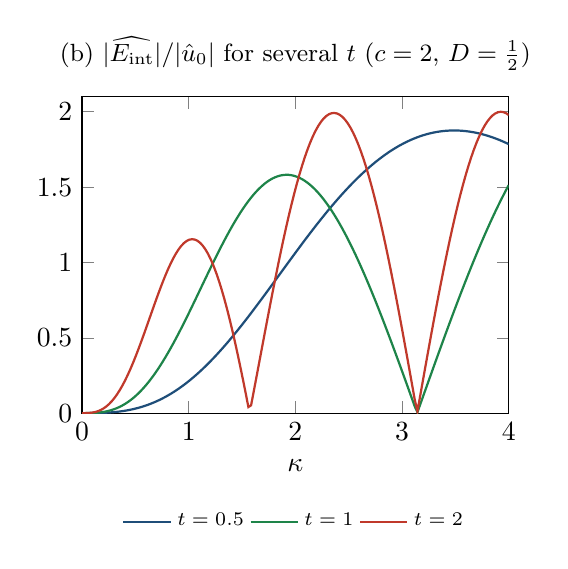
\begin{tikzpicture}
\begin{axis}[width=7.0cm,height=5.6cm,xlabel={$\kappa$},xmin=0,xmax=4,ymin=0,ymax=2.1,
 title={\small (b) $|\widehat{\Eint}|/|\hat u_0|$ for several $t$ ($c=2$, $D=\tfrac12$)},legend style={font=\scriptsize,draw=none,at={(0.5,-0.28)},anchor=north,legend columns=3},
 domain=0:4,samples=160,no markers]
\addplot[cA,thick] {sqrt(((cos(deg(2*0.5*x))-1)^2+sin(deg(2*0.5*x))^2)*(exp(-0.5*0.5*x^2)-1)^2)};
\addplot[cC,thick] {sqrt(((cos(deg(2*1.0*x))-1)^2+sin(deg(2*1.0*x))^2)*(exp(-0.5*1.0*x^2)-1)^2)};
\addplot[cB,thick] {sqrt(((cos(deg(2*2.0*x))-1)^2+sin(deg(2*2.0*x))^2)*(exp(-0.5*2.0*x^2)-1)^2)};
\legend{$t=0.5$,$t=1$,$t=2$}
\end{axis}
\end{tikzpicture}
\caption{Advection--diffusion with Gaussian datum ($\sigma^2=1$, $c=2$, $D=\tfrac12$). (a) $u_0$, $u(t)$ and $\Eint$ at $t=1$. (b) The Fourier ratio $|\widehat{\Eint}|/|\hat u_0|$ for three times.}\label{fig:eint}
\end{figure}

\subsection{Cost: $O(N)$ versus $2^N$}
Expanding \eqref{eq:eint} in the $\Delta_n$ produces one monomial per subset of $\{1,\dots,N\}$ with at least two elements: $2^N-N-1$ cross terms (Figure~\ref{fig:lattice}: the red nodes are the cross terms). Writing the \emph{complete table} of cross terms is therefore exponential. Evaluating a \emph{value} is cheap, because we never expand the product. The algorithm uses exactly the product (Fourier) form of Theorem~\ref{xthm:eint},
\[
\widehat{\Eint}(t,\kappa)=\Big[\prod_{n=1}^Ne^{ta_n(\kappa)}-1-\sum_{n=1}^N\big(e^{ta_n(\kappa)}-1\big)\Big]\hat u_0(\kappa),
\]
which for a fixed $\kappa$ needs the $N$ numbers $e^{ta_n(\kappa)}$, $N-1$ products and $N$ subtractions: $O(N)$ operations once $\hat u_0(\kappa)$ is known.
\begin{aside}{Two remarks on cost}
\textbf{What ``value'' means.} Here ``value'' means one Fourier value; recovering $\Eint(t,x)$ at a point of space needs an inverse Fourier transform, whose cost is not counted in the $O(N)$.

\textbf{Where $2^N$ comes from.} The count $2^N-N-1$ refers only to writing out all cross terms one by one; the product form never does so (Step~6 of the algorithm).
\end{aside}
\begin{figure}[!htb]
\centering
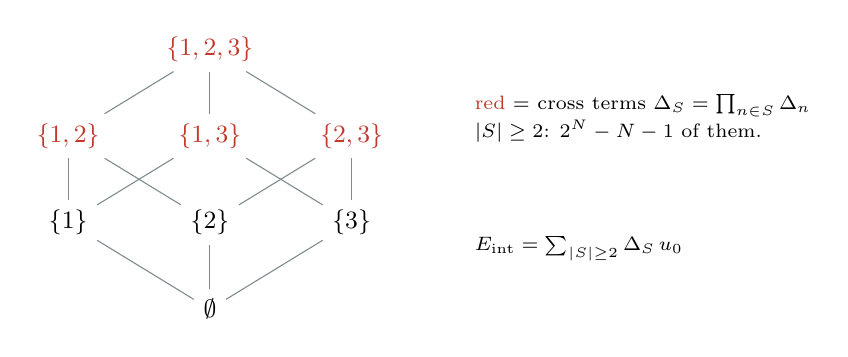
\begin{tikzpicture}[x=1.8cm,y=1.1cm,every node/.style={font=\small}]
\node (e) at (0,0) {$\emptyset$};
\node (1) at (-1,1) {$\{1\}$}; \node (2) at (0,1) {$\{2\}$}; \node (3) at (1,1) {$\{3\}$};
\node[text=cB] (12) at (-1,2) {$\{1,2\}$}; \node[text=cB] (13) at (0,2) {$\{1,3\}$}; \node[text=cB] (23) at (1,2) {$\{2,3\}$};
\node[text=cB] (123) at (0,3) {$\{1,2,3\}$};
\foreach \a/\b in {e/1,e/2,e/3,1/12,1/13,2/12,2/23,3/13,3/23,12/123,13/123,23/123} \draw[cG] (\a)--(\b);
\node[anchor=west,align=left,font=\scriptsize] at (1.8,2.2) {\textcolor{cB}{red} = cross terms $\Delta_S=\prod_{n\in S}\Delta_n$\\ $|S|\ge2$: $2^N-N-1$ of them.};
\node[anchor=west,align=left,font=\scriptsize] at (1.8,0.7) {$\Eint=\sum_{|S|\ge2}\Delta_S\,u_0$};
\end{tikzpicture}
\caption{Subset lattice for $N=3$ terms: one node per subset $S$ of terms, one monomial $\Delta_S$ per node with $|S|\ge2$. The count $2^N-N-1$ is what makes the full table exponential.}\label{fig:lattice}
\end{figure}
\begin{proposition}[{(Complexity) \led{P1-T3} \proved[]}]
In the commuting exponential-type class, a value of $\Eint$ costs $O(M(N+\sum d))$ for $M$ evaluation points; aggregated by order $O(MN^2)$; the full table $\Theta(M2^N(L+1)^2)$.
\end{proposition}
\edmark{E1}


\subsection{Time-dependent perturbation theory}
\begin{aside}{Why this subsection}
The product formula \eqref{eq:eint} needs commuting terms. When terms do not commute, or when boundary conditions are imposed, there is no closed formula, but $\Eint$ is still defined by \eqref{xeq:eint-def}. Perturbation theory expands the flow in powers of the interaction. From this expansion one reads
\begin{enumerate}[nosep,label=(\roman*)]
\item that $\Eint$ is well defined for all times (convergence),
\item approximations obtained by truncating the series order by order, and
\item the size of $\Eint$ for small $t$.
\end{enumerate}
\end{aside}

Split $A=A_1+B$, where $A_1$ is the principal term (for instance diffusion) and $B$, the remaining terms, is treated as a perturbation of $A_1$. The Dyson--Phillips series is
\begin{equation}\label{eq:dyson}
\begin{aligned}
S(t)&=\sum_{k\ge0}S^{(k)}(t),\\
S^{(0)}(t)&=e^{tA_1},\\
S^{(k+1)}(t)&=\int_0^te^{(t-s)A_1}\,B\,S^{(k)}(s)\dd s ,
\end{aligned}
\end{equation}
the same expansion that gives the interaction picture of quantum mechanics~\cite{dy}.

\begin{aside}{Reading the series}
\begin{itemize}[nosep]
\item $S^{(0)}=e^{tA_1}$ is the flow of $A_1$ alone;
\item $S^{(k)}$ collects the contributions in which $B$ acts $k$ times, at intermediate times $s\in(0,t)$, with the flow of $A_1$ in between.
\end{itemize}
The terms with $k\ge1$ are therefore the part of the flow in which $B$ acts on the evolution generated by $A_1$, that is, the interaction. (When $A_1$ and $B$ commute, the first-order term is
\[
\int_0^te^{(t-s)A_1}Be^{sA_1}\dd s=t\,Be^{tA_1},
\]
consistent with Section~\ref{sec:inside}.)
\end{aside}

\textbf{What it gives.} The series converges for all $t$ when $A_1$ generates an even-order dissipative semigroup (e.g.\ diffusion) and $B$ is a lower-order $L^\infty$ perturbation, also with Dirichlet conditions \led{P3-T1} \modulo{Miyadera--Voigt~\cite{en}}: so $\Eint$ is well defined and can be approximated by truncation even without a closed formula. Each $S^{(k)}$ is the order-$k$ part of the interaction. For small times, for boundary-induced interaction, with $k$ the order of contact of the datum with the boundary, $\|\Eint\|\sim t^{k/2+3/4}$ \led{P3-T3, OP-F5A} \proved\edmark{E10}: the smoother the datum is against the boundary (larger $k$), the faster the interaction becomes negligible as $t\to0$.

\subsection{Non-commuting terms}\label{sec:noncomm}
If $[A_1,A_2]\ne0$, then $e^{t(A_1+A_2)}\neq e^{tA_1}e^{tA_2}$; by Baker--Campbell--Hausdorff,
\[
e^{tA_1}e^{tA_2}=\exp\!\Big(t(A_1+A_2)+\tfrac{t^2}{2}[A_1,A_2]+O(t^3)\Big).
\]
\begin{proposition}[{(Lie-algebra dichotomy) \led{P1-T4, P1-T5} \proved[]}]
If the Lie algebra generated by the terms is solvable, an exact formula with finitely many scalar functions exists (Wei--Norman). Otherwise only a local expansion exists, and \textbf{no finite product of the flows of the individual terms} reproduces $e^{t(X+\varepsilon Y)}$.
\end{proposition}
\begin{takeaway}
For commuting terms the interaction is explicit and cheap to evaluate, but it cannot be made to vanish nor be computed stably in $H^m$; for non-commuting terms even the explicit form is lost in general. These are the linear-case limits against which the nonlinear extension of Section~\ref{sec:nonlin} must be read.
\end{takeaway}

%======================================================================


\section{When does a solution determine its equation?}\label{sec:identify}
\inbrief{The identification criterion, uniqueness, and what finite data can and cannot certify. This explains why the algorithm of the companion paper never reports ``identified''.}
% Shared module: identification, uniqueness, the spectral form, limits of certification.
\subsection{When does a solution determine its equation?}\label{sec:ident}
Let $\Omega$ be open and connected (on a disconnected set the pieces may obey different equations),
let $u\in\mathcal D'(\Omega)$ satisfy $P(\partial)u=0$, and let $P=\prod_iP_i^{e_i}$ (up to a nonzero constant factor) be the
factorization of $P$ into pairwise non-associate irreducible polynomials $P_i$ with multiplicities
$e_i$. The question is whether $\Ann(u)=(P)$: then every constant-coefficient equation satisfied by
$u$ is a consequence of $P$, and $P$ is determined by $u$.

\begin{theorem}[Identification criterion]\label{thm:ident}
Put $v_i=(P/P_i)(\partial)\,u$ and $v_i'=(P/P_i^{e_i})(\partial)\,u$.
\begin{enumerate}[label=(\alph*)]
  \item $\Ann(u)=(P)$ if and only if $v_i\notin\EP(\Omega)$ for every $i$.
  \item $\Var(\Ann u)=\Var(P)$ if and only if $v_i'\notin\EP(\Omega)$ for every $i$.
  \item If $P$ is square-free, (a) and (b) coincide. If $P$ is monic in $\tau$ of degree $m$, then
  $\Ann(u)=(P)$ if and only if the only $(\varphi_0,\dots,\varphi_{m-1})\in\C[\xi]^m$ with
  $\sum_{j<m}\varphi_j(\partial_x)\,\partial_t^{\,j}u=0$ is zero.
\end{enumerate}
\end{theorem}

The idea is to strip one irreducible factor and look at what is left. The function $v_i$ solves
$P_i(\partial)v_i=0$. If $v_i$ is a generic solution of that factor, no smaller operator kills $u$.
If $v_i$ is an exponential-polynomial, some $h$ coprime to $P_i$ kills it, and then
$h\cdot P/P_i$ is an annihilator of $u$ that is not a multiple of $P$. The converse uses
\cref{lem:gcd}; the full proof is in \cref{app:proofs}.

\begin{proposition}[Uniqueness and the intrinsic operator]\label{prop:unique}
\begin{enumerate}[label=(\alph*)]
  \item If $\Ann(u)=(P)$, then $P$ is determined by $u$ up to a nonzero constant and is the unique
  annihilator of minimal degree.
  \item $\Ann(u)=(P)$ if and only if $\sigp(u)=\emptyset$ and $\Gu\sim P$ (equality up to a constant).
  \item For any annihilator $P$, the multiplicity of $P_i$ in $\Gu$ equals $e_i-\max\{k\le e_i:
  (P/P_i^{k})(\partial)u\in\EP\}$. Hence $\Gu$ is computed from any annihilator by at most
  $\sum_ie_i$ membership tests ``$\in\EP$''.
\end{enumerate}
\end{proposition}

\begin{example}[The heat equation, continued]\label{ex:heat-ident}
For $P=\tau-\nu\xi^2$ (irreducible) the criterion reads: $\Ann(u)=(P)$ if and only if $u\notin\EP$.
One mode $e^{-\nu\kappa^2t+i\kappa x}$ has $\Ann(u)=(\tau+\nu\kappa^2,\ \xi-i\kappa)$, a point of
$\Var(P)$; it cannot distinguish the heat equation from the pure decay $\partial_t+\nu\kappa^2$, or from
any other equation whose variety passes through the point $(-\nu\kappa^2,i\kappa)$. The heat kernel is not in $\EP$, so every
constant-coefficient equation it satisfies is a multiple of $\partial_t-\nu\partial_x^2$.
\end{example}

\begin{remark}[Curves and points]\label{rem:curves-points}
The two cases of \cref{ex:heat-ident} sit at the two ends of the decomposition~\eqref{eq:GJ}. A finite sum of modes
$u\in\EP$ has an annihilator with finitely many zeros, so
\[
  u\in\EP:\qquad \Gu=1,\qquad \sigp(u)=\{(\tau_j,\xi_j)\}\ \text{finite (its exponents)},
\]
whereas the zero set of a nonconstant polynomial in two variables is a whole algebraic curve. For the heat kernel
the situation is reversed:
\[
  u=t^{-1/2}e^{-x^2/(4\nu t)}:\qquad \Gu=\tau-\nu\xi^2,\quad \Var(\Gu)\ \text{a curve},\qquad \sigp(u)=\emptyset .
\]
By \cref{prop:unique}(b) it is exactly this pair, an empty point spectrum together with $\Gu\sim P$, that gives
$\Ann(u)=(P)$: the solution fills the whole curve of its equation and contains no isolated mode besides.
\end{remark}

\roleinalg{Data never contain the heat kernel, they contain finitely many sampled modes; a finite
set of modes is always an exponential-polynomial. The algorithm therefore never claims that an
equation is \emph{identified}. It asks whether the modes it sees are \emph{compatible} with a factored
symbol and are rich enough in each factor (enough distinct wavenumbers per branch) for the factor to
be pinned down within its class. This is the meaning of the label \FC{} in the companion algorithm paper.}

\subsection{What finite data can and cannot certify}\label{sec:certify}
\Cref{thm:ident} speaks about $u$, not about finitely many numbers. Two facts frame what an algorithm
can promise.

Recall that $\ring u=\spn\{\partial_t^{\,j}\partial_x^{\,k}u:\ j,k\ge0\}$ is the vector space generated by the
derivatives of $u$ (\cref{sec:ep}). The \emph{jet} of order $M$ of $u$ at a point $z_0=(t_0,x_0)$ is the list of its
derivatives of order at most $M$ at that point; for example
\[
  j^2_{z_0}(u)=\big(u,\ u_t,\ u_x,\ u_{tt},\ u_{tx},\ u_{xx}\big)\big|_{(t,x)=z_0}.
\]

\begin{proposition}[Finite data]\label{prop:certify}
Let $\Omega$ be connected and $z_0\in\Omega$.
\begin{enumerate}[label=(\roman*)]
  \item If $\dim_\C\ring u\le n$, the jet of order $2n-1$ of $u$ at $z_0$ determines $\Ann(u)$ among all functions
  $u'$ with $\dim_\C\ring u'\le n$.
  \item For every $u$ and every $M$ there is a polynomial, hence an exponential-polynomial, with the same jet of
  order $M$ at $z_0$; and for finitely many sample points there is an exponential-polynomial with the same values.
  Consequently, without a bound on $\dim\ring u$, no finite set of jets or samples proves $\Ann(u)=(P)$.
\end{enumerate}
\end{proposition}

\begin{proof}
(ii) The Taylor polynomial of order $M$ at $z_0$ has the same jet, and polynomial interpolation in two variables
matches any finite set of values. Both are exponential-polynomials, and an exponential-polynomial never has
$\Ann=(P)$ when $P$ has an irreducible factor (\cref{thm:ident}: all $v_i$ are then exponential-polynomials).
(i) The space $\ring u$ is invariant under differentiation and, by \cref{lem:ep}, consists of real-analytic
exponential-polynomials. Let $K_M$ be the subspace of elements of $\ring u$ whose jet of order $M$ vanishes at $z_0$.
Then $K_{M+1}=\{f\in K_0:\ \partial_tf,\partial_xf\in K_M\}$, so once $K_{M+1}=K_M$ the chain is constant, and a
constant $K_M$ is a derivative-invariant space of functions vanishing at $z_0$ with all their derivatives, hence
$\{0\}$. Since $\dim K_0\le n-1$, the chain reaches $\{0\}$ by $M=n-1$: the jet of order $n-1$ at $z_0$ is injective
on $\ring u$, and likewise on $\ring u'$. For $Q$ of degree at most $n$, $Q\in\Ann(u)$ iff the jet of order
$n-1$ of $Q(\partial)u$ vanishes at $z_0$, a condition on the jet of order $2n-1$ of $u$; the same holds for $u'$.
Finally $\Ann(u)$ has codimension at most $n$, so a Gr\"obner basis for a degree-compatible order consists of
polynomials of degree at most $n$; the same holds for $\Ann(u')$, and two ideals generated in degree at most $n$
that contain the same polynomials of degree at most $n$ are equal.
\end{proof}

The consequence for learning is a design rule: without an a priori bound on $\dim\ring u$, which data never
supply, an algorithm can refute a candidate equation, or report that it is compatible with the data at
the resolution available, but it cannot certify it. Its output must carry a label that says which of these
happened.


\section{Nonlinear equations}\label{sec:nonlin}
\inbrief{The same two questions, asked of Burgers-type equations: the interaction term for the flows of single terms, behaviour before, at and after a shock, and identification relative to a dictionary.}
\sectionbrief
{a scalar equation in one space variable, $u_t=\sum_nT_n(u)$, each $T_n$ linear or polynomial in the jet $(u,u_x,u_{xx},\dots)$; $\Omega$ bounded and simply connected; the exact solution is known.}
{to test which of the notions of Sections~\ref{sec:ident}--\ref{sec:inside} survive when the terms are nonlinear.}
{extension of the chain. \emph{Result:} weaker, relative statements (exact expansion of $\Eint$, sharp asymptotics across a shock for Burgers, identification relative to a dictionary). Benchmarks: Burgers, KdV--Burgers, Fisher--KPP; KdV and NLS only as controls.}
We consider $u_t=\sum_nT_n(u)$ with each $T_n$ linear or polynomial in the jet $(u,u_x,u_{xx},\dots)$. Benchmarks: Burgers $u_t=-uu_x+\nu u_{xx}$, KdV--Burgers, Fisher--KPP; integrable cases (KdV, NLS) serve as controls.

\subsection{Interaction term for flows of single terms}
With $S_n$ the (nonlinear) flow of $u_t=T_n(u)$ alone, \eqref{xeq:eint-def} still defines $\Eint^{\mathrm{add}}$. Its Taylor expansion in $t$:
\begin{theorem}[{(Jet expansion) \led{S4T-T1} \proved[]}]\label{thm:jet}
$\displaystyle \Eint^{\mathrm{add}}=\frac{t^2}{2}\sum_{n\ne m}T_n'[\,T_m(u_0)\,]+O(t^3)$, where $T_n'[v]$ is the Fr\'echet derivative of $T_n$ at $u_0$ in the direction $v$.
\end{theorem}
\begin{example}[Burgers]\label{ex:burgers-jet}
$T_1=-uu_x$, $T_2=\nu u_{xx}$. Then $T_1'[v]=-(vu_x+uv_x)$ and $T_2'[v]=\nu v_{xx}$, so
\[
\begin{aligned}
T_1'[T_2u_0]&=-\nu\,(u_0''u_0'+u_0u_0'''),\\
T_2'[T_1u_0]&=-\nu\,(3u_0'u_0''+u_0u_0'''),
\end{aligned}
\]
and half the sum times $t^2$ gives
\[
\begin{aligned}
\Eint&=\tfrac12\big(T_1'[T_2u_0]+T_2'[T_1u_0]\big)t^2+O(t^3)\\
&=-\nu\big(u_0u_0'''+2u_0'u_0''\big)t^2+O(t^3).
\end{aligned}
\]
\end{example}

\subsection{Before, at, and after the shock}
The interaction term of Burgers changes qualitatively with time, and each regime calls for different tools:
\begin{description}[nosep,leftmargin=3.2cm,labelwidth=3.0cm]
\item[Before shock formation] smoothness permits perturbative expansions and derivative-based estimates.
\item[At breaking] the inviscid gradient blows up, invalidating estimates that require smoothness.
\item[After shock formation] pointwise behavior can be discontinuous, so $L^1$ estimates become more informative than pointwise bounds.
\end{description}
Figure~\ref{fig:burgers} recalls why a shock appears at all in the flow of the single term $-uu_x$: along each characteristic $u$ is constant and the characteristic moves with speed $u$, so faster parts overtake slower ones. For $u_0=\sin x$ the characteristics are
\[
x=\xi+t\sin\xi
\]
(the parameter $s$ in the figure plays the role of the time $t$); since
\[
\frac{\partial x}{\partial\xi}=1+t\cos\xi
\]
vanishes first at $\xi=\pi$, the breaking time is $t^*=1$.
\begin{figure}[!htb]
\centering
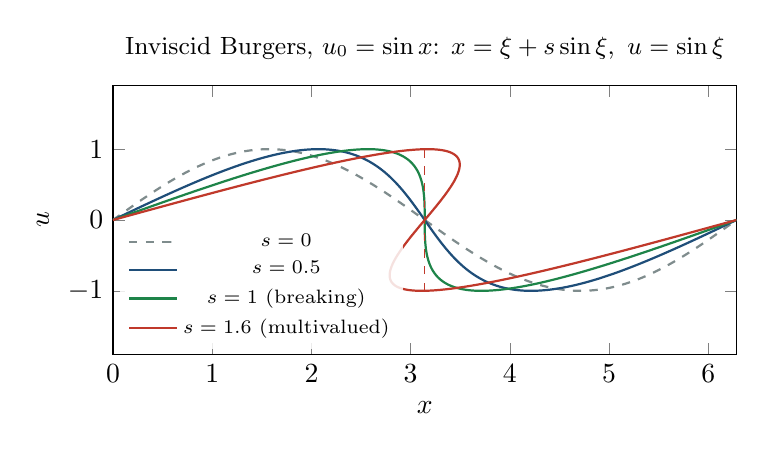
\begin{tikzpicture}
\begin{axis}[width=9.5cm,height=5.0cm,xlabel={$x$},ylabel={$u$},xmin=0,xmax=6.283,ymin=-1.9,ymax=1.9,
 legend style={font=\scriptsize,draw=none,fill=white,fill opacity=0.85,text opacity=1,at={(0.01,0.02)},anchor=south west},
 title={\small Inviscid Burgers, $u_0=\sin x$: $x=\xi+s\sin\xi,\ u=\sin\xi$},no markers,domain=0:6.283185,samples=200,smooth]
\addplot[cG,thick,dashed,variable=\z] ({\z},{sin(deg(\z))});
\addplot[cA,thick,variable=\z] ({\z+0.5*sin(deg(\z))},{sin(deg(\z))});
\addplot[cC,thick,variable=\z] ({\z+1.0*sin(deg(\z))},{sin(deg(\z))});
\addplot[cB,thick,variable=\z] ({\z+1.6*sin(deg(\z))},{sin(deg(\z))});
\draw[cB,dashed] (axis cs:3.14159,-1) -- (axis cs:3.14159,1);
\legend{$s=0$,$s=0.5$,$s=1$ (breaking),$s=1.6$ (multivalued)}
\end{axis}
\end{tikzpicture}
\caption{Characteristic solution of the inviscid flow of $-uu_x$. At $s=1$ the profile has a vertical tangent: the gradient blows up. Beyond that the curve folds; the physical (entropy) solution replaces the fold by a jump at $x=\pi$ (equal-area rule), shown dashed. This breaking is what makes $\Eint$ discontinuous after the shock.}\label{fig:burgers}
\end{figure}
\paragraph{Before the shock ($t<t^*$): smooth regime.} Smoothness permits perturbative expansions and derivative-based estimates.
\begin{itemize}[nosep]
\item $\Eint$ has a closed form at first order in $\nu$, with remainder $O(\nu^2\varepsilon^2t^3)$ \led{S4T-T2} \proved; it blows up at the breaking time $t^*$ \led{S4T-P3}. (This is the same family of expansions as Theorem~\ref{thm:jet} and Example~\ref{ex:burgers-jet}.)
\item The Cole--Hopf substitution $u=-2\nu\varphi_x/\varphi$ turns Burgers into the heat equation $\varphi_t=\nu\varphi_{xx}$; the inverse scattering transform linearizes KdV and NLS. These are used as the ``exact linearization'' of the nonlinear solution~\cite{ch}.
\end{itemize}
\paragraph{At breaking ($t=t^*$): estimates that need smoothness fail.} The inviscid gradient $u_x$ blows up (vertical tangent, $s=1$ in Figure~\ref{fig:burgers}), so every statement that needs bounds on $u_x,u_{xx},\dots$ stops being usable at $t^*$: the closed form of $\Eint$ blows up, and estimates that require smoothness, such as those behind the jet expansion of Theorem~\ref{thm:jet}, are no longer valid.
\paragraph{After the shock ($t>t^*$): discontinuous regime.}
The flow of $-uu_x$ alone forms a shock, so $\Eint$ jumps by amounts independent of $\nu$; this is forced by the definition. A function with a jump is not in $H^1$ in one dimension, so the Sobolev norms of Sections~\ref{sec:groups} and~\ref{sec:inside} are no longer the natural ones: pointwise values are unreliable, while the \emph{measure} of the discrepancy is well behaved. The meaningful quantities are therefore $L^1$ sizes, collected below:
\begin{align}
\|\Eint\|_{L^1}&=\Theta(\nu),\\
\sup_{t\le T}\|\Eint\|_{L^1}&=\nu|\log\nu|+O(\nu),\\
\|S-S_1S_2\|_{L^1}&=\Theta(\sqrt\nu).
\end{align}
The first line holds at fixed $t$, each shock contributing $4\nu\log\!\big(2\cosh(\rho/2)\big)$; the second has exact leading coefficient $1$. Sources: the first line is \led{OPA-T1} \modulo{Kru\v zkov uniqueness~\cite{kr}}; the second is \led{OPF5A-T1/T2}; the third is \led{OPF5D-T6} \proved.
The second line holds for data with a single birth of shock such as $\sin x$, and is conditional on a localization lemma in general \condl{}.

\begin{table}[!htb]
\centering\small
\begin{tabular}{@{}L{3.0cm}L{4.9cm}L{6.2cm}@{}}
\toprule
Regime & What happens & Tools and results\\\midrule
Before the shock, $t<t^*$ & the profile is smooth, characteristics do not cross & jet expansion (Thm.~\ref{thm:jet}), first-order closed form of $\Eint$, Cole--Hopf\\
At breaking, $t=t^*$ & the inviscid gradient blows up (vertical tangent) & smoothness-based estimates fail; $\Eint$ blows up\\
After the shock, $t>t^*$ & the single-term flow is discontinuous (equal-area rule) & $L^1$ estimates: $\Theta(\nu)$, $\nu|\log\nu|$, $\Theta(\sqrt\nu)$\\
\bottomrule
\end{tabular}
\caption{The three regimes of the Burgers interaction term and the tools that apply in each.}\label{tab:regimes}
\end{table}

\subsection{Identification relative to a dictionary}
Nonlinear terms cannot be handled by the ideal $\Ann(u)$ of Section~\ref{sec:theory}; instead one fixes a finite candidate list. Choose a dictionary $\mathcal D$ of monomials of degree $\le d$ in the jet, of order $\le k$, and ask which polynomial relations $F(u,u_x,\dots)=0$ the data satisfy. Notation: $V$ is the span of $\mathcal D$, $I(u)$ the ideal of all differential relations satisfied by $u$, $[F]$ the differential ideal generated by $F$, and $\mathcal J_u$ the jet-level obstruction (a different object from the cofactor $J_u$ of Section~\ref{sec:theory}, hence the calligraphic letter)\edmark{E13}.
\begin{theorem}[{(Dictionary criterion) \led{S4ID-T1} \proved[]}]\label{thm:dict}
For smooth $u$ on any $\Omega$ there is an exact sequence $0\to[F]\cap V\to I(u)\cap V\to\mathcal J_u\cap\psi(V)\to0$. In particular
\[
I(u)\cap V=[F]\cap V\iff\mathcal J_u\cap\psi(V)=0 .
\]
\end{theorem}
The correct statement is therefore ``the relations are exactly $F$ \emph{modulo its differential consequences}''; the literal ``$I(u)\cap V=\langle F\rangle$'' is false in complete dictionaries (they contain $\partial_xF$, etc.) \led{S4ID-P1}. Concrete criteria: for Burgers with $N$ shocks, $u$ identifies the equation in the evolutionary dictionary iff $d\le N$ \led{S4ID-T2, OP-T7}; for $N$-soliton KdV the identifying polynomial has total degree $(N+2)2^{N-1}$ (generic $N=2$: $8$) \led{OP-K15} \modulo{Novikov 1974~\cite{no}}. Finally, ``closed form $\Rightarrow$ does not identify'' is itself a theorem \led{S4ID-T4}.
\edmark{E2}

\subsection{Linear versus nonlinear: the same idea, two structures}
Sections~\ref{sec:theory}--\ref{sec:inside} and the present one answer the same question: \emph{what does a single solution $u$ remember about its equation?} In both settings we collect all relations satisfied by $u$ and ask when these relations are generated by the equation we were given. What changes is the algebraic structure in which the relations live.
\begin{table}[!htb]
\centering\small
\begin{tabular}{@{}L{2.8cm}L{6.2cm}L{6.2cm}@{}}
\toprule
 & Linear approach (Sections~\ref{sec:theory}--\ref{sec:inside}) & Nonlinear approach (this section)\\\midrule
Space of candidate equations & the ring $\ring=\C[\tau,\xi]$ of constant-coefficient operators & a finite \emph{dictionary} $\mathcal D$ of jet monomials of degree $\le d$ and order $\le k$; $V=\spn\mathcal D$\\
Relations satisfied by $u$ & $\Ann(u)$, an ideal of $\ring$ & $I(u)$, the ideal of all differential relations\\
What the equation generates & the principal ideal $(P)$ & the differential ideal $[F]$\\
Criterion for identification & $\Ann(u)=(P)$ (Theorem~\ref{thm:ident}) & $I(u)\cap V=[F]\cap V$, i.e.\ $F$ \emph{modulo its differential consequences} (Theorem~\ref{thm:dict})\\
What escapes the equation & the cofactor $J_u$: the finitely many exponentials in $u$ ($\sigma_p(u)=\Var(J_u)$) & the jet-level obstruction $\mathcal J_u\cap\psi(V)$ (exact sequence of Theorem~\ref{thm:dict})\\
Solutions that do not identify & $u\in\EP$ & closed-form solutions (\led{S4ID-T4})\\
Concrete criteria & finite linear algebra (Lemma~\ref{lem:ep}) & Burgers with $N$ shocks identifies iff $d\le N$; $N$-soliton KdV: degree $(N+2)2^{N-1}$\\
\bottomrule
\end{tabular}
\caption{The linear and nonlinear identification problems side by side.}\label{tab:lin-nonlin}
\end{table}
\begin{aside}{Where the parallel breaks}
\textbf{Linear case.} The solutions form a vector space and the annihilators an ideal: one can add, multiply by operators and factor, which is why the Nullstellensatz applies and the test is a finite-dimensional computation.

\textbf{Nonlinear case.} There is no linear structure on the solutions: one must fix a finite space $V$ of candidates in advance, and the identification is \emph{relative to $V$}, never absolute. The literal statement
\[
I(u)\cap V=\langle F\rangle
\]
is false in complete dictionaries, which contain $\partial_xF$, so the correct statement is ``modulo differential consequences''.
\end{aside}

\begin{keypoint}
Both approaches ask what one solution determines about its equation. The linear one answers with the annihilator ideal $\Ann(u)$ and its generator $G_u$; the nonlinear one answers with a dictionary and the differential ideal of relations, and only up to differential consequences. In the algorithm of the companion paper Steps~1--6 use the structure of $\Ann(u)$, while Step~7 switches to the dictionary and returns a relative identification.
\end{keypoint}

%======================================================================


\section{Limits, open problems, and status}\label{sec:limits}
% Shared: the kinds of claim (proved / design rule / measured).
\begin{table}[tbp]
\centering\small
\caption{The kinds of claim made in the paper.}\label{tab:status}
\begin{tabularx}{\linewidth}{@{}>{\raggedright\arraybackslash}p{2.2cm}X@{}}
\toprule
Kind & Statements\\
\midrule
proved & groups are factors with overlap $\deltaP$ (\cref{thm:factor}); terms are not groups (\cref{prop:terms,prop:discont});
identification criterion and its limits on finite data (\cref{thm:ident,prop:unique,prop:certify}); stability via
$\gN$ (\cref{thm:hm}); Bayesian error bars via the angle (the companion algorithm paper); counting condition\\
design rule & labels instead of ``identified''; distributions of $\rho$ instead of values; decisions on the raw observations;
growth of the class instead of coefficient penalties; minimum-norm split of the overlap\\
measured & $0/20$ confident wrong answers on random equations not used in development; $60/60$ factor sets on grid
designs with independent fields and noise; $30/30$ on the development benchmark; coefficient coverage $0.94$ at
nominal $0.90$\\
\bottomrule
\end{tabularx}
\end{table}

\sectionbrief
{no new assumptions.}
{to state what is impossible, what is open, and how reliable the results are.}
{delimits the claims of the paper.}
\paragraph{What is impossible} (all \proved).
\begin{itemize}[nosep]
\item finite certificates of identification, and black-box identification (Section~\ref{sec:certify});
\item per-term decomposition of the solution (Proposition~\ref{prop:terms}\edmark{E9});
\item stable regularization of $\Eint$ (Proposition~\ref{prop:discont});
\item identification by restricting variable-coefficient operators to one solution;
\item decomposition on domains with holes (Figure~\ref{fig:hole});
\item a finite product of single-term flows reproducing non-commuting dynamics.
\end{itemize}

\paragraph{Open or conditional.}
\begin{itemize}[nosep]
\item identification for analytic KdV data with nonzero reflection coefficient \led{INT-Q1} \openq;
\item time-uniform shock estimate with several shock births \led{OPA-Q1} \condl;
\item density of the sum of kernels on nonconvex domains \openq;
\item exact values $\delta_N(K)$ of an invariant for general $N$ \led{OPF5C-Q1} \openq;
\item nonlinear asymptotics with derivatives \led{S4ID-P8} \condl;
\item closedness of the sum of kernels for $N\ge3$ differential factors \led{C12-Q2} \openq.
\end{itemize}

\paragraph{Honest assessment.} Many ingredients are classical (Malgrange--Ehrenpreis, Nullstellensatz, Cole--Hopf, inverse scattering). The contribution is the \emph{package}: sharp characterizations, negative theorems, and counterexamples, each with a verified status. Independent reviewers were AI agents. Fifteen theorems of the algebraic core (the $\Eint$ identity for commuting flows, the comaximal factor decomposition with explicit projector, companion normality for $k=2$, irreducibility results) are formalized in Lean~4/Mathlib without \texttt{sorry}; the analytic parts (distributions, Sobolev spaces, semigroups) are not, since Mathlib lacks the libraries. Several citations were verified only on secondary sources; a result relied upon should be traced to its primary source. Out of scope so far: a variable potential treated as noise (Schr\"odinger/Dirac), matrix-valued coefficients ($4\times4$ Dirac), and any statistical preprocessing.

%======================================================================
\clearpage


\appendix
% Shared appendix: proofs of the results of the analytical part.
\section{Proofs}\label{app:proofs}
Throughout, $\Omega\subset\R^2$ is open and connected, $\mathcal A$ is $\mathcal D'(\Omega)$ or $C^\infty(\Omega)$, and
$\ring=\C[\tau,\xi]$ acts on $\mathcal A$ by $\tau\mapsto\partial_t$, $\xi\mapsto\partial_x$. For $z=(\tau_z,\xi_z)\in\C^2$,
$\mathfrak m_z=(\tau-\tau_z,\xi-\xi_z)$ is its maximal ideal and $\psi_z(t,x)=e^{\tau_zt+\xi_zx}$.

\subsection{Algebraic toolkit}
\begin{proof}[Proof of \cref{lem:gcd}]
\emph{Coprime polynomials meet in finitely many points.} Let $f,g\ne0$ be coprime. By Gauss's lemma they are
coprime in the principal ideal domain $\C(\xi)[\tau]$, so $af+bg=1$ there; clearing denominators,
$a'f+b'g=r(\xi)\ne0$ with $a',b'\in\ring$. At a common zero $r(\xi_0)=0$, which leaves finitely many $\xi_0$;
exchanging the variables, finitely many $\tau_0$. Hence $\Var(f,g)$ is finite.

\emph{Splitting.} Put $J=\{f/g:\ f\in I\}$ with $g=\gcdop(I)$; it is an ideal and $I=gJ$, and no prime divides all
of $J$. If $J\ne\ring$, pick $0\ne f\in J$ with distinct prime factors $\pi_1,\dots,\pi_r$ and, for each $a$,
$g_a\in J$ with $\pi_a\nmid g_a$. The sets $\{c\in\C^r:\pi_a\mid\sum_bc_bg_b\}$ are proper linear subspaces, so some
$c$ avoids all of them; then $f$ and $\sum_bc_bg_b\in J$ are coprime and $\Var(J)\subseteq\Var(f,\sum_bc_bg_b)$ is
finite. By the Nullstellensatz a power of $\sqrt J$ lies in $J$, and $J=\ring$ when $\Var(J)=\emptyset$.
\end{proof}

\begin{proof}[Proof of \cref{lem:ep}]
($\Rightarrow$) $Q(\partial)(q\,\psi_z)=\big(Q(z+\partial)q\big)\psi_z$ for every polynomial $q$, so the derivatives of
$q\,\psi_z$ stay in the finite-dimensional space of polynomials of degree $\le\deg q$ times $\psi_z$. Moreover
$\prod_k\mathfrak m_{z_k}^{\deg q_k+1}\subseteq\Ann(w)$, so $\Var(\Ann w)\subseteq\{z_k\}$; conversely
$Q\in\Ann(w)$ forces $Q(z_k+\partial)q_k=0$ by the linear independence of distinct exponentials, whose top-degree part
is $Q(z_k)$ times that of $q_k$, so $Q(z_k)=0$.

($\Leftarrow$) Let $\ring w$ be finite-dimensional and $p,q$ the minimal polynomials of $\partial_t$ and
$\partial_x$ restricted to $\ring w$, so that $p(\partial_t)w=0$ and $q(\partial_x)w=0$. On an open rectangle $I'\times J'\subset\Omega$, induction
on $\deg p$ shows that every distribution with $p(\partial_t)v=0$ is $\sum_{j,l}c_{jl}(x)\,t^le^{\lambda_jt}$ with
$c_{jl}\in\mathcal D'(J')$ and $\lambda_j$ the roots of $p$ (the base case uses that a distribution with
$\partial_tV=0$ on a rectangle is $c(x)\otimes1$). Applying $q(\partial_x)$ and testing against functions dual to
$t^le^{\lambda_jt}$ gives $q(\partial_x)c_{jl}=0$, so each $c_{jl}$ is an exponential-polynomial of $x$. Thus $w$ is an
exponential-polynomial $E$ near every point. The set where $w$ coincides near $y$ with a fixed $E$ is open, and it is
closed because two exponential-polynomials that agree on an open set agree everywhere; by connectedness it is
$\Omega$.
\end{proof}

\subsection{Identification}
\begin{proof}[Proof of \cref{thm:ident}]
Let $I=\Ann(u)\ni P$ and write $I=G\,J$ as in \cref{lem:gcd}. Since $P\in I$, $G\mid P$, so
$G=c'\prod_iP_i^{f_i}$ with $0\le f_i\le e_i$. First, $G\sim P$ iff $I=(P)$: if $G\sim P$ then
$I=PJ\subseteq(P)\subseteq I$; if $I=(P)$, $P$ divides all of $I$ and lies in $I$.

(a), $\Leftarrow$ by contraposition. If $I\ne(P)$, some $f_i<e_i$, so $P/P_i=G\,H$ with $H\in\ring$. A power
$\mathfrak n^{\ell}$ of the ideal $\mathfrak n$ of the finite set $\Var(J)$ lies in $J$, and for $h\in\mathfrak n^{\ell}$,
$h\cdot P/P_i=G(Hh)\in GJ=I$, i.e.\ $h(\partial)v_i=0$. So $\Var(\Ann v_i)\subseteq\Var(J)$ is finite and
$v_i\in\EP$ by \cref{lem:ep}.

(a), $\Rightarrow$ by contraposition. If $v_i\in\EP$, $\Var(\Ann v_i)$ is finite while $\Var(P_i)$ is infinite, so
some $h\in\Ann(v_i)$ is not divisible by $P_i$. Then $Q=h\cdot P/P_i$ satisfies $Q(\partial)u=h(\partial)v_i=0$; if
$Q=PA$, cancelling $P/P_i$ gives $h=P_iA$, a contradiction. So $Q\in I\setminus(P)$.

(b) $\Var(I)=\Var(G)\cup\Var(J)$ with $\Var(J)$ finite. If $f_i\ge1$, $\Var(P_i)\subseteq\Var(I)$; if $f_i=0$,
$\Var(P_i)\cap\Var(I)$ lies in the finite set $\bigcup_{f_j\ge1}\Var(P_i,P_j)\cup\Var(J)$, so
$\Var(P_i)\not\subseteq\Var(I)$. Hence $\Var(I)=\Var(P)$ iff all $f_i\ge1$, and $f_i=0$ iff $v_i'\in\EP$ by the
argument of (a) with $P/P_i^{e_i}$ in place of $P/P_i$.

(c) If $e_i=1$ then $v_i=v_i'$. If $P$ is monic of degree $m$ in $\tau$, divide any $Q\in\ring$ by $P$ in
$\C[\xi][\tau]$: $Q=AP+\sum_{j<m}\varphi_j(\xi)\tau^j$ uniquely. Then $Q\in I$ iff $\sum_j\varphi_j(\partial_x)\partial_t^ju=0$, and
$Q\in(P)$ iff all $\varphi_j=0$.
\end{proof}

\begin{proof}[Proof of \cref{prop:unique}]
(a) If $I=(P)$, every annihilator is $SP$ and $\deg SP\ge\deg P$ with equality iff $S$ is a nonzero constant.
(b) If $I=(P)$ then $G\sim P$ and $J=\ring$, so $\sigp(u)=\emptyset$. Conversely, $\Var(J)=\emptyset$ gives $J=\ring$ by
the Nullstellensatz, hence $I=(G)=(P)$. (c) Let $f_i$ be the multiplicity of $P_i$ in $G$ and $w=(P/P_i^k)(\partial)u$. If $k\le e_i-f_i$, then
$G\mid P/P_i^k$, say $P/P_i^k=GH$; for $h$ in a power $\mathfrak n^{\ell}\subseteq J$ of the ideal of $\Var(J)$,
$h\cdot P/P_i^k=G(Hh)\in I$, so $\Ann(w)\supseteq\mathfrak n^{\ell}$ and $w\in\EP$. If $k>e_i-f_i$ and $w\in\EP$, pick
$h\in\Ann(w)$ with $P_i\nmid h$ (as in the proof of \cref{thm:ident}); then $hP/P_i^k\in I$, so $G\mid hP/P_i^k$, but
$P_i$ occurs in $hP/P_i^k$ with multiplicity $e_i-k<f_i$, a contradiction. Hence
$f_i=e_i-\max\{k:\ w\in\EP\}$.
\end{proof}

\subsection{Decomposition and stability}
\begin{proof}[Proof of \cref{thm:factor}]
We prove the statement for open connected $\Omega$ with $H^1_{dR}(\Omega)=0$, which holds for simply connected domains.

\emph{Step 1: finite modules have no obstruction.} Let $M$ be an $\ring$-module of finite dimension over $\C$. Then
$\operatorname{Ext}^1_\ring(M,\mathcal A)=0$ and $\dim\operatorname{Hom}_\ring(M,\mathcal A)=\dim M$. By the long exact sequence it is
enough to check one-dimensional modules $\ring/\mathfrak m_z$, since $M$ has a composition series with such
quotients. A free resolution of $\ring/\mathfrak m_z$ is the Koszul complex of $(\tau-\tau_z,\xi-\xi_z)$, so
$\operatorname{Ext}^\bullet(\ring/\mathfrak m_z,\mathcal A)$ is the cohomology of
$\mathcal A\to\mathcal A^2\to\mathcal A$, $v\mapsto\big((\partial_t-\tau_z)v,(\partial_x-\xi_z)v\big)$, $(a,b)\mapsto(\partial_t-\tau_z)b-(\partial_x-\xi_z)a$.
Multiplication by $\psi_{-z}$ turns it into the de Rham complex of $\Omega$ with coefficients in $\mathcal A$, whose first
cohomology is $H^1_{dR}(\Omega)=0$ (for distributions by de Rham's theorem), and whose zeroth cohomology is the constants,
of dimension one.

\emph{Step 2: two factors.} For coprime $Q_1,Q_2$, $(Q_1)\cap(Q_2)=(Q_1Q_2)$ by unique factorization, and
$0\to\ring/(Q_1Q_2)\to\ring/(Q_1)\oplus\ring/(Q_2)\to\ring/(Q_1,Q_2)\to0$ is exact ($1\mapsto(1,1)$, $(a,b)\mapsto a-b$).
Applying $\operatorname{Hom}_\ring(\cdot,\mathcal A)$, and using $\operatorname{Hom}(\ring/(f),\mathcal A)=\ker_{\mathcal A}f$,
gives the exact sequence
$0\to\operatorname{Hom}(\ring/(Q_1,Q_2),\mathcal A)\to\ker Q_1\oplus\ker Q_2\xrightarrow{(u_1,u_2)\mapsto u_1+u_2}\ker Q_1Q_2\to
\operatorname{Ext}^1(\ring/(Q_1,Q_2),\mathcal A)$. The quotient $\ring/(Q_1,Q_2)$ is finite-dimensional by
\cref{lem:gcd}, so by Step~1 the last group vanishes: the sum map is onto, and its kernel has dimension
$\dim\ring/(Q_1,Q_2)$ and consists of solutions of a zero-dimensional ideal, i.e.\ of exponential-polynomials.

\emph{Step 3: induction.} $P'=Q_2\cdots Q_N$ is coprime to $Q_1$, so $\ker P=\ker Q_1+\ker P'$, and by induction
$\ker P'=\sum_{j\ge2}\ker Q_j$. Dimensions of kernels add along the composition of the two sum maps, and
$\dim\ring/(Q_1,P')=\sum_{j\ge2}\dim\ring/(Q_1,Q_j)$ because $\ring/(Q_1,Q_2Q_3\cdots)$ is the direct sum of its
localizations at the finitely many common zeros, where the intersection multiplicities add. This gives
\eqref{eq:deltaP}.
\end{proof}

\begin{proof}[Proof of \cref{thm:hm}]
The sum operator $\sumop$ is bounded from $\bigoplus_jM_j$ into $\ker_{\Hs}P$, and every $u$ in its range has
components in $\Hs$. Its range is all of $\ker_{\Hs}P$ iff the range is closed and dense. By the closed range theorem the
range is closed iff $\sumop$ is bounded below on $(\ker\sumop)^\perp$, i.e.\ iff $\gN>0$, and then the minimum-norm
preimage satisfies \eqref{eq:stability}. For two closed subspaces, $M_1+M_2$ is closed iff $\cF<1$, and
$\gamma_2=1-\cF$~\cite{Deu01}. In finite dimension every subspace sum is closed, and the sum equals the span of
the sampled exponentials of $P$, each of which lies in the kernel of one factor.
\end{proof}

\begin{proof}[Proof of \cref{prop:discont}]
For real $\zeta>c/\nu$ let $u_\zeta=e^{\lambda_\zeta t+\zeta x}$, $\lambda_\zeta=\nu\zeta^2-c\zeta>0$; then $Q(\partial)u_\zeta=0$ and
$\norm{u_\zeta}_{\Hs(\Omega)}\le C_s(1+\zeta)^{2s}e^{\lambda_\zeta T}\norm{e^{\zeta x}}_{L^2(a,b)}$. With base time $t_0$ and horizon
$t$, \cref{thm:eint} gives
\[
  \Eint=e^{\lambda_\zeta t_0}\big(e^{-c\zeta t}-1\big)\big(e^{\nu\zeta^2t}-1\big)\,e^{\zeta x},
\]
whose $L^2(\Omega)$ norm is at least a constant times $e^{\nu\zeta^2t}\norm{e^{\zeta x}}_{L^2(a,b)}$ for large $\zeta$. With
$t_0=0$ and $t=T$ the ratio therefore grows at least like
\[
  e^{\nu\zeta^2T-\lambda_\zeta T}(1+\zeta)^{-2s}=e^{c\zeta T}(1+\zeta)^{-2s},
\]
which is unbounded for every $s$. For the second statement, $v+w$ is killed by $Q$ and by
$R=(\tau+c\xi)(\tau-\nu\xi^2)$. At a common zero of $Q$ and $R$, either $\tau=-c\xi$, and then $Q=0$ gives
$\nu\xi^2=0$, or $\tau=\nu\xi^2$, and then $c\xi=0$; in both cases $(\tau,\xi)=(0,0)$. So $(Q,R)$ has a single zero, and
its common kernel is a finite-dimensional space of exponential-polynomials (\cref{lem:ep}).
\end{proof}


\section{Primer for readers new to the concepts}\label{app:primer}
This appendix \emph{adds} concrete explanations; nothing in the main text depends on reading it. It covers four notions in this order: ideals and annihilators (\S B.1), exponential-polynomials (\S B.2), the Chinese remainder theorem (\S B.3), and the companion matrix on a numerical example (\S B.4).

\subsection*{B.1 Ideals, annihilators and the gcd, starting from integers}
\paragraph{Integers.} The multiples of $6$ form an \emph{ideal} $(6)=\{\dots,-6,0,6,12,\dots\}$: it is closed under addition and under multiplication by any integer. The ideal generated by $4$ and $6$ is $(4,6)=(2)$, since $2=6-4$ and every combination is even: the ideal ``remembers'' only the $\gcd$.

\paragraph{Operators.} Replace integers by operators and ``multiple of $6$'' by ``kills $u$''. For $u=e^{x}$ every operator $Q(\partial_x)$ with $Q(1)=0$ kills $u$, i.e.\ every multiple of $\partial_x-1$. So
\[
\begin{aligned}
\Ann(e^x)&=(\partial_x-1),\\
\Ann(\sin x)&=(\partial_x^2+1),\\
\Ann(xe^x)&=\big((\partial_x-1)^2\big),\\
\Ann(e^x+e^{2x})&=\big((\partial_x-1)(\partial_x-2)\big).
\end{aligned}
\]
In one variable every annihilator ideal has a single generator (the \emph{minimal annihilator}), exactly as every ideal of integers is $(n)$. In two variables an ideal can need several generators, as $(\tau-\tau_0,\xi-\xi_0)$ does for $u=e^{\tau_0t+\xi_0x}$.

\paragraph{The gcd.} $\Ann(u)=G_uJ_u$ separates the part of the ideal that is a single polynomial multiple ($G_u$, ``infinite part'') from the part $J_u$ that has only finitely many common zeros ($J_u$, ``finite debris''). Example: for $u=f(x+t)$ with $f$ generic (not an exponential-polynomial), $\Ann(u)=(\partial_t-\partial_x)$ by Theorem~\ref{thm:ident}, so $G_u=\tau-\xi$ and $J_u=\ring$; for $u=e^{x+t}$, $\Ann(u)=(\tau-1,\xi-1)$, so $G_u=1$ and $J_u=\Ann(u)$.

\subsection*{B.2 Exponential-polynomials: examples and a test}
\begin{center}\small
\begin{tabular}{@{}L{5.4cm}L{2.3cm}L{6.8cm}@{}}
\toprule
Function & In $\EP$? & Reason (derivatives of $u$ span ...)\\\midrule
$xe^{x}$ & yes & $\spn\{xe^x,e^x\}$, dimension $2$\\
$x^2e^{3t}+\cos x$ & yes & finite sum of polynomial $\times$ exponential ($\cos x=\tfrac12(e^{ix}+e^{-ix})$)\\
$e^{-x^2}$ (Gaussian) & no & $\frac{d^k}{dx^k}e^{-x^2}=(\text{polynomial of degree }k)\,e^{-x^2}$: independent for all $k$, infinite dimension\\
$1/(1+x^2)$ & no & derivatives are rational functions with growing denominators: infinite dimension\\
\bottomrule
\end{tabular}
\end{center}
This is Lemma~\ref{lem:ep} in action: ``$u\in\EP$'' means ``its derivatives span a finite-dimensional space''.

\subsection*{B.3 The Chinese remainder theorem, concretely}
\paragraph{Integers.} The system $x\equiv1\pmod2$, $x\equiv2\pmod3$ has the unique solution $x\equiv5\pmod6$: $\Z/6\cong\Z/2\times\Z/3$. Coprimality of $2$ and $3$ is what makes the pair of remainders determine $x$.

\paragraph{One-variable ODE.} Let $p(\partial)=(\partial-1)(\partial-2)$. Then $\ker p=\ker(\partial-1)\oplus\ker(\partial-2)=\spn\{e^x,e^{2x}\}$, and the Lagrange-type projectors are explicit: if $u=ae^x+be^{2x}$,
\[
\begin{aligned}
u_1&=\frac{\partial-2}{1-2}\,u=\;\;a\,e^{x},\\
u_2&=\frac{\partial-1}{2-1}\,u=\;\;b\,e^{2x}.
\end{aligned}
\]
This is Eq.~\eqref{xeq:lagrange} with $\partial_t$ replaced by $\partial$.

\paragraph{Two variables.} For the wave equation $Q_1=\tau-\xi$, $Q_2=\tau+\xi$ are coprime, but the ideal $(Q_1,Q_2)=(\tau,\xi)$ is not the unit ideal: the two lines meet at the origin. The quotient $\ring/(\tau,\xi)=\C$ has dimension $1$, which is the constant ambiguity $\delta(P)=1$ of the wave equation. Theorem~\ref{thm:factor} says that this finite overlap is the \emph{only} failure of the integer picture.

\subsection*{B.4 The companion matrix on a numerical example}
For $u''-3u'+2u=0$ the companion matrix is $C=\begin{pmatrix}0&1\\-2&3\end{pmatrix}$, with characteristic polynomial $\lambda^2-3\lambda+2$ and eigenvalues $1,2$. The projectors of Eq.~\eqref{eq:spectral} are $\Pi_1=\dfrac{C-2\Id}{1-2}$ and $\Pi_2=\dfrac{C-\Id}{2-1}$, and $e^{xC}=e^x\Pi_1+e^{2x}\Pi_2$.



\IfFileExists{siamplain.bst}{\bibliographystyle{siamplain}}{\bibliographystyle{plain}}
\bibliography{../shared/refs,refs_extra}
\end{document}
